\documentclass{beamer}
\usepackage[english]{babel}
\usepackage{amsmath,amssymb,graphicx}

%%%%%%%%%% Start TeXmacs macros
\catcode`\<=\active \def<{
\fontencoding{T1}\selectfont\symbol{60}\fontencoding{\encodingdefault}}
\catcode`\>=\active \def>{
\fontencoding{T1}\selectfont\symbol{62}\fontencoding{\encodingdefault}}
\newcommand{\mathd}{\mathrm{d}}
\newcommand{\nospace}{}
\newcommand{\tmfoldedstd}[2]{\trivlist{\item[$\bullet$]\mbox{}#1}}
\newcommand{\tmmathbf}[1]{\ensuremath{\boldsymbol{#1}}}
\newcommand{\tmop}[1]{\ensuremath{\operatorname{#1}}}
\newcommand{\nonconverted}[1]{\mbox{}}
%%%%%%%%%% End TeXmacs macros

\begin{document}

{\screens{\begin{frame}
  \
  
  \
  
  \
  
  \
  
  \
  
  \title{计算视觉与模式识别}
  
  \maketitle
  
  \ 
\end{frame}}{\begin{frame}
  \frametitle{线性滤波器}
  
  \ 
\end{frame}}{\begin{frame}
  \frametitle{线性滤波与卷积}
  
  平均值:
  \begin{eqnarray*}
    \mathcal{R}_{i \nospace j} & = & \frac{1}{(2 k + 1)^2} \sum_{u = i - k}^{u
    = i + k} \sum_{v = j - k}^{v = j + k} \mathcal{F}_{u \nospace v}
  \end{eqnarray*}
  卷积:
  \begin{eqnarray*}
    \mathcal{R}_{i \nospace j} & = & \sum_{u, v} H_{i - u, j - v} F_{u, v}
  \end{eqnarray*}
\end{frame}}{\begin{frame}
  \frametitle{均值滤波示例}
  
  {\hspace{7em}}\resizebox{0.5\columnwidth}{!}{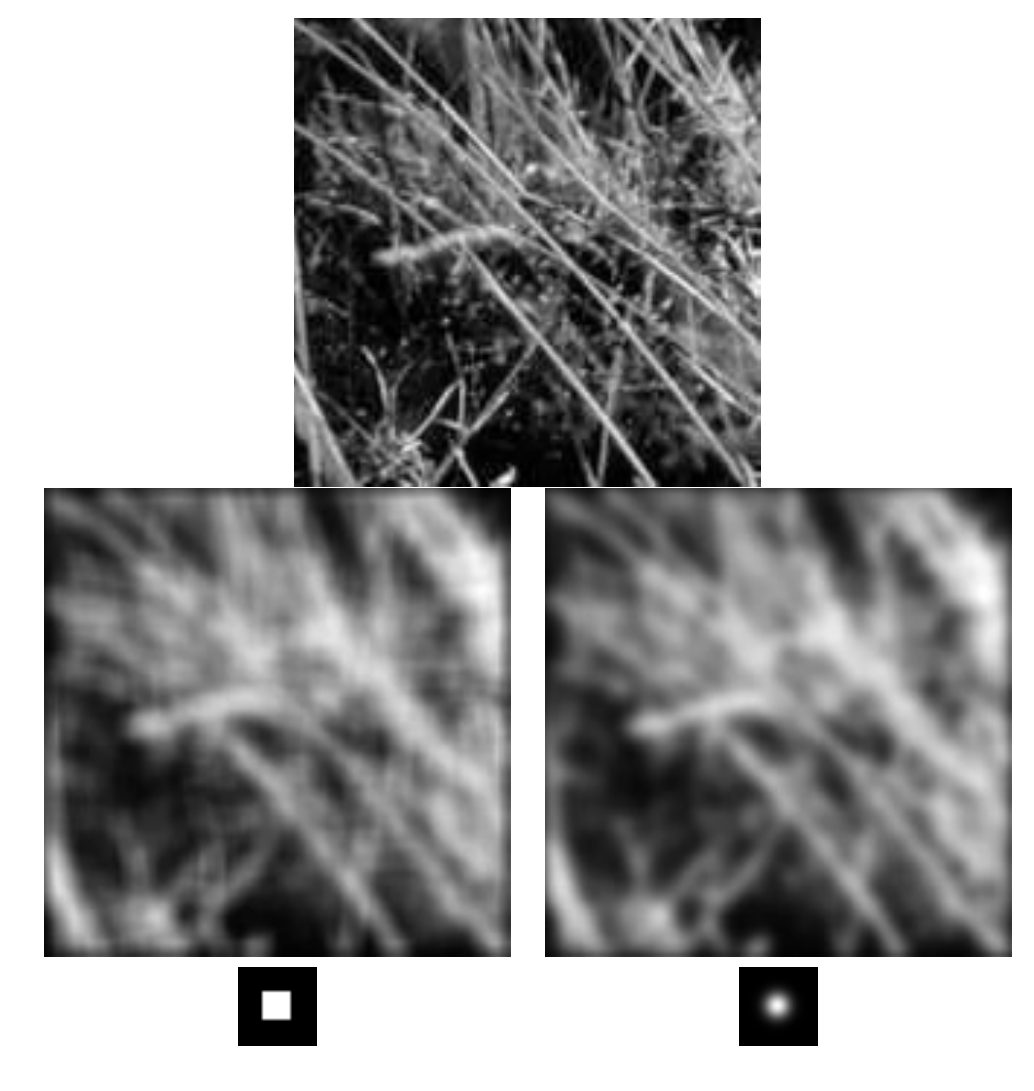
\includegraphics{img/uniform_weighted_average.png}}
  
  \tmfoldedstd{Figure 8.1.}{Although a uniform local average may seem to give
  a good blurring model, it generates effects that are not usually seen in
  defocussing a lens. The images above compare the effects of a uniform local
  average with weighted average. The image at the top shows a view of grass.
  On the left in the second row, the result of blurring this image using a
  uniform local model and on the right, the result of blurring this image
  using a set of Gaussian weights. The degree of blurring in each case is
  about the same, but the uniform average produces a set of narrow vertical
  and horizontal bars --- an effect often known as ringing. The bottom row
  shows the weights used to blur the image, themselves rendered as an image;
  bright points represent large values and dark points represent small values
  (in this example the smallest values are zero).}
\end{frame}}{\begin{frame}
  \frametitle{高斯核}
  
  \
  
  对称高斯核:
  \begin{eqnarray*}
    G_{\sigma} (x, y) & = & \frac{1}{2 \pi \sigma^2} \exp \left( - \frac{(x^2
    + y^2)}{2 \sigma^2} \right)
  \end{eqnarray*}
  离散形式,$2 k + 1 \times 2 k + 1$矩阵:
  \begin{eqnarray*}
    H_{i \nospace j} & = & \frac{1}{2 \pi \sigma^2} \exp \left( - \frac{((i -
    k - 1)^2 + (j - k - 1)^2)}{2 \sigma^2} \right)
  \end{eqnarray*}
\end{frame}}{\begin{frame}
  \frametitle{高斯核}
  
  {\hspace{4em}}\resizebox{0.7\columnwidth}{!}{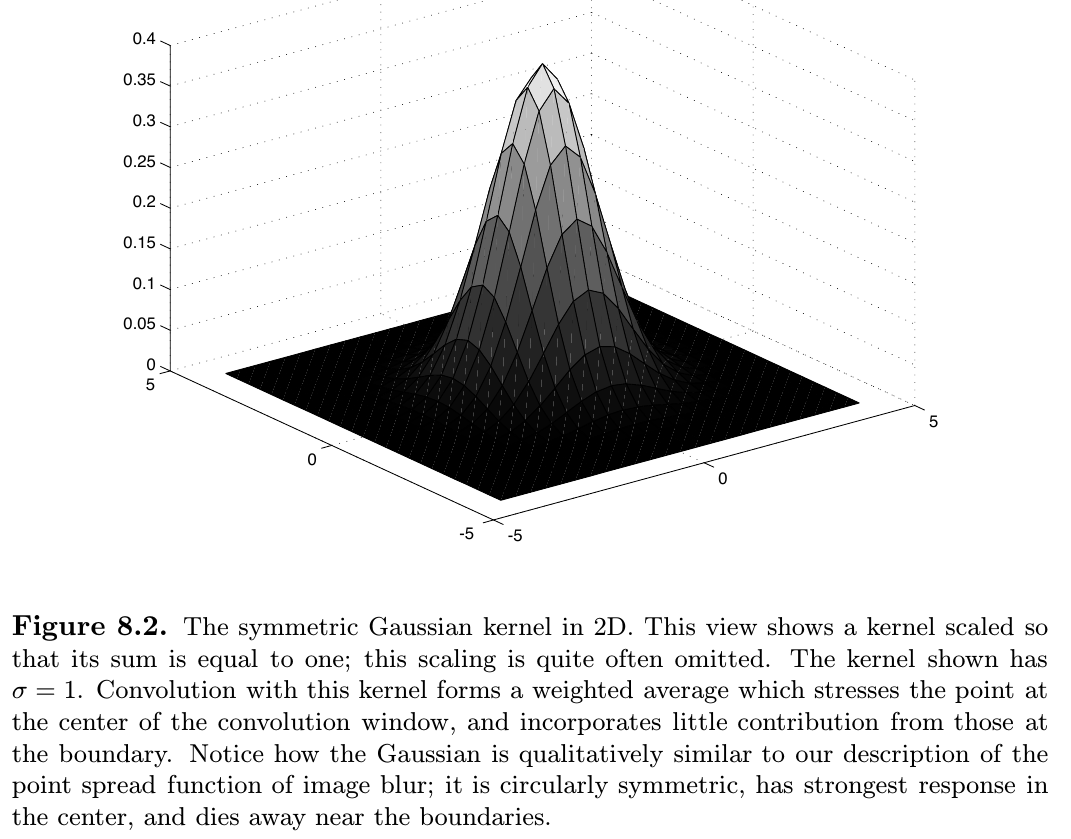
\includegraphics{img/gaussian_kernel.png}}
\end{frame}}{\begin{frame}
  \frametitle{高斯噪声与高斯滤波器}
  
  {\hspace{4em}}\resizebox{0.6\columnwidth}{!}{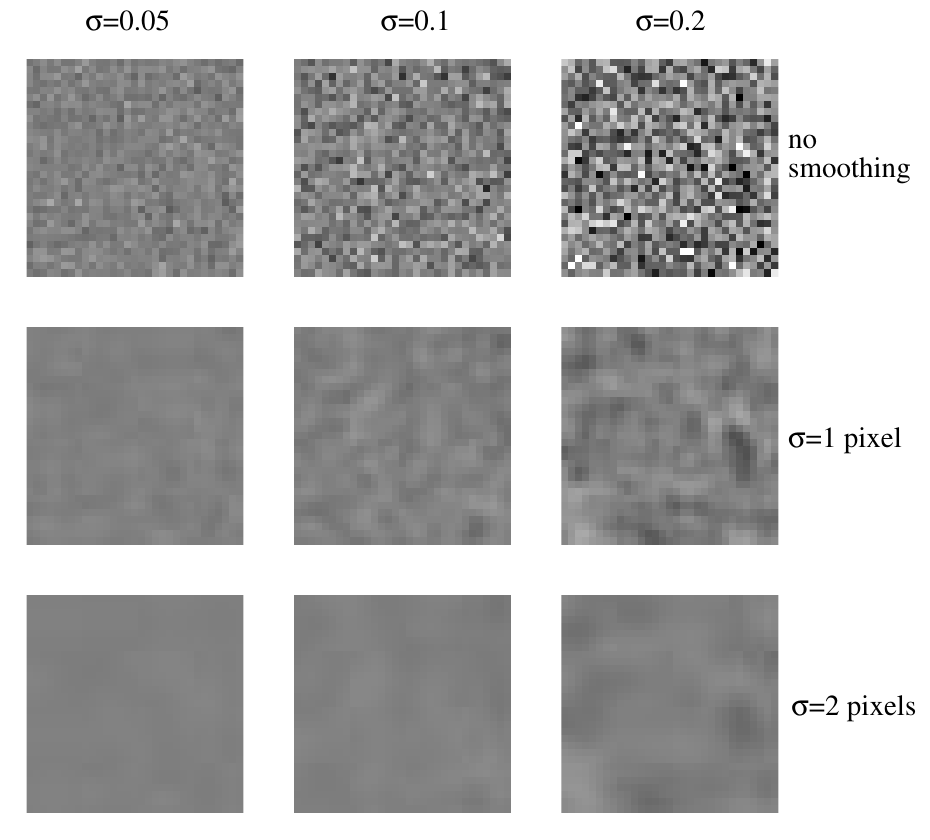
\includegraphics{img/gaussian_noise_filter.png}}
  
  \tmfoldedstd{FIGURE 4.3:}{The top row shows images of a constant mid-gray
  level corrupted by additive Gaussian noise. In this noise model, each pixel
  has a zero-mean normal random variable added to it. The range of pixel
  values is from zero to one, so that the standard deviation of the noise in
  the first column is about 1/20 of full range. The center row shows the
  effect of smoothing the corresponding image in the top row with a Gaussian
  filter of {\sigma} one pixel. Notice the annoying overloading of notation
  here; there is Gaussian noise and Gaussian filters, and both have
  {\sigma}'s. One uses context to keep these two straight, although this is
  not always as helpful as it could be, because Gaussian filters are
  particularly good at suppressing Gaussian noise. This is because the noise
  values at each pixel are independent, meaning that the expected value of
  their average is going to be the noise mean. The bottom row shows the effect
  of smoothing the corresponding image in the top row with a Gaussian filter
  of {\sigma} two pixels.
  
  \ }
\end{frame}}{\begin{frame}
  \frametitle{椒盐噪声与高斯滤波}
  
  {\hspace{7em}}\resizebox{0.5\columnwidth}{!}{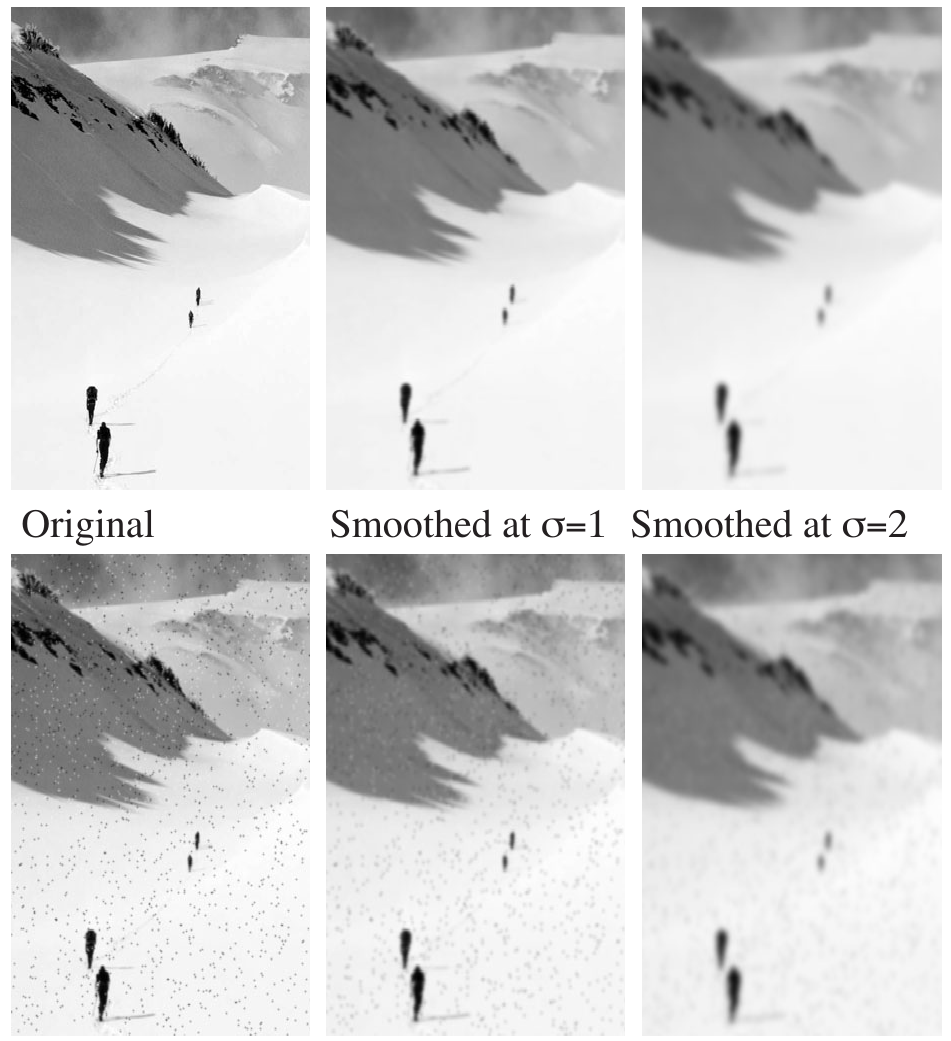
\includegraphics{img/salt_pepper_gaussian_filter.png}}
  
  \tmfoldedstd{Figure 8.3.}{ In salt-and-pepper noise, we choose pixels
  uniformly at random, and uni-formly at random make them either black or
  white. Gaussian smoothing is particularly effective at suppressing the
  effects of salt-and-pepper noise. The top row shows an image, and versions
  smoothed by a symmetric Gaussian with {\sigma} two pixels and four pixels.
  The images in the second row are obtained by corrupting the images in the
  top row by this noise model and then smoothing the result. Notice that, as
  the smoothing increases, detail is lost, but the effects of the noise
  diminish, too --- the smoothed versions of the noisy images look very much
  like the smoothed version of the noise-free images.
  
  \ }
\end{frame}}{\begin{frame}
  \frametitle{导数与有限差分}
  
  偏导数
  \begin{eqnarray*}
    \frac{\partial f}{\partial x} & = & \lim_{\varepsilon \rightarrow 0}
    \frac{f (x + \varepsilon, y) - f (x, y)}{\varepsilon}
  \end{eqnarray*}
  有限差分
  \begin{eqnarray*}
    \frac{\partial h}{\partial x} & \approx & h_{i + 1, j} - h_{i - 1, j}
  \end{eqnarray*}
  卷积核
  \begin{eqnarray*}
    \mathcal{H} & = & \left\{ \begin{array}{lll}
      0 & 0 & 0\\
      1 & 0 & - 1\\
      0 & 0 & 0
    \end{array} \right\}
  \end{eqnarray*}
\end{frame}}{\begin{frame}
  \frametitle{差分图像}
  
  {\hspace{3em}}\resizebox{0.8\columnwidth}{!}{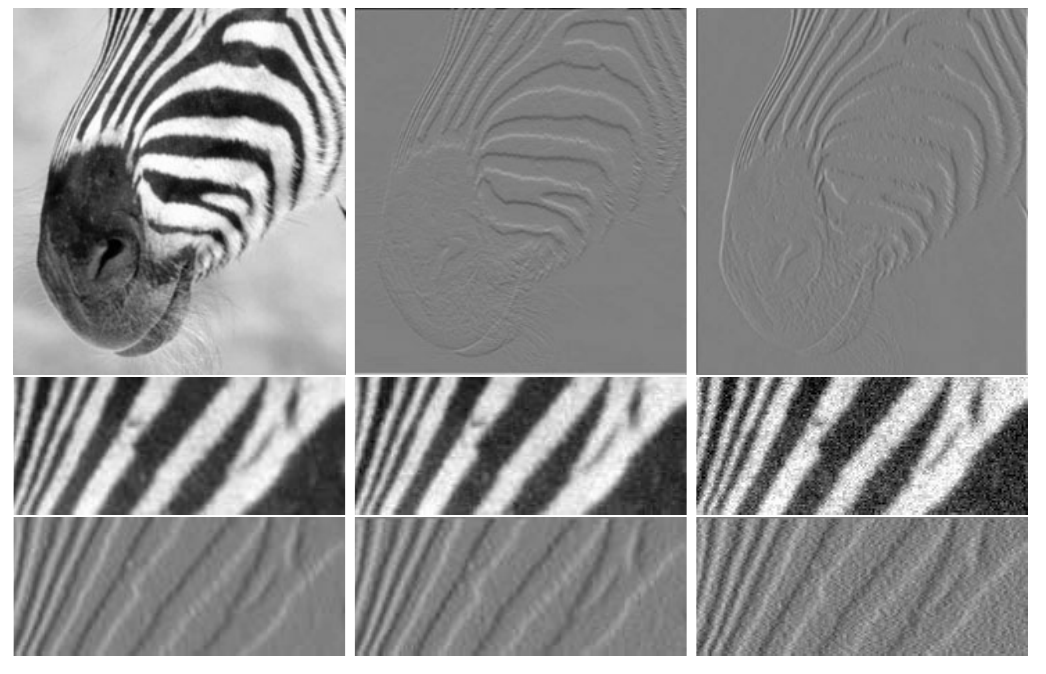
\includegraphics{img/difference_image_zebra.png}}
  
  \tmfoldedstd{FIGURE 4.4:}{The top row shows estimates of derivatives
  obtained by finite differences. The image at the left shows a detail from a
  picture of a zebra. The center image shows the partial derivative in the
  y-direction---which responds strongly to horizontal stripes and weakly to
  vertical stripes---and the right image shows the partial derivative in the
  x-direction---which responds strongly to vertical stripes and weakly to
  horizontal stripes. However, finite differences respond strongly to noise.
  The image at center left shows a detail from a picture of a zebra; the next
  image in the row is obtained by adding a random number with zero mean and
  normal distribution ({\sigma} = 0.03; the darkest value in the image is 0,
  and the lightest 1) to each pixel; and the third image is obtained by adding
  a random number with zero mean and normal distribution ({\sigma} = 0.09) to
  each pixel. The bottom row shows the partial derivative in the x-direction
  of the image at the head of the row. Notice how strongly the differentiation
  process emphasizes image noise; the derivative figures look increasingly
  grainy. In the derivative figures, a mid-gray level is a zero value, a dark
  gray level is a negative value, and a light gray level is a positive value.
  
  \ }
\end{frame}}{\begin{frame}
  \frametitle{平移不变线性系统}
  
  线性
  \begin{eqnarray*}
    R (f + g) & = & R (f) + R (g)\\
    R (k \nospace f) & = & k \nospace R (f)
  \end{eqnarray*}
  平移不变
  \begin{eqnarray*}
    R (f (x)) & = & g (x)\\
    R (f (x - y)) & = & g (x - y)
  \end{eqnarray*}
\end{frame}}{\begin{frame}
  \frametitle{离散卷积}
  \begin{eqnarray*}
    \tmmathbf{e}_0 & = & \ldots .0, 0, 0, 1, 0, 0, 0 \ldots .\\
    \tmmathbf{f} & = & \sum_i f_i \tmop{Shift} (\tmmathbf{e}_0, i)\\
    R (\tmop{Shift} (\tmmathbf{f}, k)) & = & \tmop{Shift} (R (\tmmathbf{f}),
    k)\\
    R (k\tmmathbf{f}) & = & k \nospace R (\tmmathbf{f})
  \end{eqnarray*}
  \begin{eqnarray*}
    R (\tmmathbf{f}) & = & R \left( \sum_i f_i \tmop{Shift} (\tmmathbf{e}_0,
    i) \right)\\
    & = & \sum_i R (f_i \tmop{Shift} (\tmmathbf{e}_0, i))\\
    & = & \sum_i f_i R (\tmop{Shift} (\tmmathbf{e}_0, i))\\
    & = & \sum_i f_i \tmop{Shift} (R (\tmmathbf{e}_0), i)
  \end{eqnarray*}
\end{frame}}{\begin{frame}
  \frametitle{离散卷积(续)}
  \begin{eqnarray*}
    \tmmathbf{g} & = & R (\tmmathbf{e}_0)\\
    R (\tmmathbf{f}) & = & \sum_i f_i \tmop{Shift} (\tmmathbf{g}, i)\\
    & = & \tmmathbf{g} \ast \tmmathbf{f}\\
    R_j & = & \sum_i g_{j - i} f_i
  \end{eqnarray*}
\end{frame}}{\begin{frame}
  \frametitle{二维卷积}
  \begin{eqnarray*}
    \mathcal{E}_{00} & = & \begin{array}{lll}
      0 & 0 & 0\\
      0 & 1 & 0\\
      0 & 0 & 0
    \end{array}\\
    R_{i \nospace j} & = & \sum_{u, v} G_{i - u, j - v} F_{u \nospace v}\\
    \mathcal{R} & = & \mathcal{G} \ast \ast \mathcal{H}
  \end{eqnarray*}
\end{frame}}{\begin{frame}
  \frametitle{连续卷积}
  \begin{eqnarray*}
    R (k \nospace f) & = & k \nospace R (f)\\
    \tmop{Shift} (f, c) & = & f (u - c)\\
    R (\tmop{Shift} (f, c)) & = & \tmop{Shift} (R (f), c)\\
    \tmop{box}_{\varepsilon} (x) & = & \left\{\begin{array}{ll}
      0 & \tmop{abs} (x) > \frac{\varepsilon}{2}\\
      1 & \tmop{abs} (x) < \frac{\varepsilon}{2}
    \end{array}\right.\\
    R \left( \sum_i f_i \tmop{Shift} (\tmop{box}_{\varepsilon}, x_i) \right) &
    = & \sum_i R (f_i \tmop{Shift} (\tmop{box}_{\varepsilon}, x_i))\\
    & = & \sum_i f_i R (\tmop{Shift} (\tmop{box}_{\varepsilon}, x_i))\\
    & = & \sum_i f_i \tmop{Shift} \left( R \left(
    \frac{\tmop{box}_{\varepsilon}}{\varepsilon} \varepsilon \right), x_i
    \right)\\
    & = & \sum_i f_i \tmop{Shift} \left( R \left(
    \frac{\tmop{box}_{\varepsilon}}{\varepsilon} \right), x_i \right)
    \varepsilon
  \end{eqnarray*}
\end{frame}}{\begin{frame}
  \frametitle{连续卷积(续)}
  
  $\delta$函数
  \begin{eqnarray*}
    d_{\varepsilon} (x) & = & \frac{\tmop{box}_{\varepsilon}
    (x)}{\varepsilon}\\
    \delta (x) & = & \lim_{\varepsilon \rightarrow 0} d_{\varepsilon} (x)
  \end{eqnarray*}
  卷积
  \begin{eqnarray*}
    R (f) & = & \int \{ R (\delta (u - x')) \} f (x') \mathd x'\\
    & = & \int g (u - x') f (x') \mathd x'\\
    & = & (g \ast f)\\
    (g \ast f) & = & (h \ast g)\\
    (f \ast (g \ast h)) & = & ((f \ast g) \ast h)
  \end{eqnarray*}
\end{frame}}{\begin{frame}
  \frametitle{二维卷积}
  \begin{eqnarray*}
    d_{\varepsilon} (x, y) & = & \frac{\tmop{box}_{\varepsilon^2} (x,
    y)}{\varepsilon^2}\\
    R (h) & = & \int \int g (x - x', y - y') h (x', y') \mathd x \mathd y\\
    & = & (g \ast \ast h)\\
    (g \ast \ast h) & = & (h \ast \ast g)
  \end{eqnarray*}
\end{frame}}{\begin{frame}
  \frametitle{傅里叶变换}
  
  
  \begin{eqnarray*}
    \mathcal{F} (g (x, y)) & = & \int \int g (x, y) e^{- i 2 \pi (u \nospace x
    + v \nospace y)} \mathd x \mathd y\\
    e^{\nonconverted{minus} i 2 \pi (u \nospace x + v \nospace y)} & = & \cos
    (2 \pi (u \nospace x + v \nospace y)) + i \nospace \sin (2 \pi (u \nospace
    x + v \nospace y))
  \end{eqnarray*}
  线性
  \begin{eqnarray*}
    \mathcal{F} (g + h) & = & \mathcal{F} (g) +\mathcal{F} (h)\\
    \mathcal{F} (k \nospace g (x, y)) & = & k\mathcal{F} (g (x, y))
  \end{eqnarray*}
  反变换
  \begin{eqnarray*}
    g (x, y) & = & \int \int \mathcal{F} (g) e^{i 2 \pi (u \nospace x + v
    \nospace y)} \mathd u \mathd v
  \end{eqnarray*}
\end{frame}}{\begin{frame}
  \frametitle{傅里叶基实部示例}
  
  \resizebox{1\columnwidth}{!}{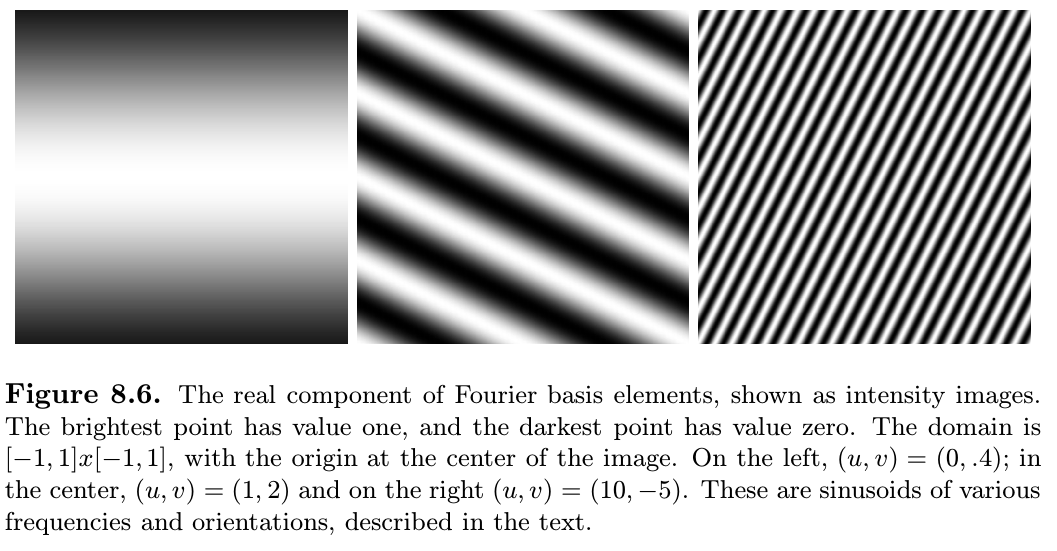
\includegraphics{img/fourier_base.png}}
\end{frame}}{\begin{frame}
  \frametitle{幅值与相位}
  \begin{eqnarray*}
    \mathcal{F} (g (x, y)) & = & \int \int g (x, y) \cos (2 \pi u \nospace x +
    v \nospace y) \mathd x \mathd y\\
    &  & + i \int \int g (x, y) \sin (2 \pi u \nospace x + v \nospace y)
    \mathd x \mathd y\\
    & = & \mathfrak{R} (\mathcal{F} (g)) + i \ast \mathfrak{F} (\mathcal{F}
    (g))\\
    & = & \mathcal{F}_R (g) + i \ast \mathcal{F}_I (g)
  \end{eqnarray*}
\end{frame}}{\begin{frame}
  \frametitle{傅里叶变换示例}
  
  {\hspace{3em}}\resizebox{0.8\columnwidth}{!}{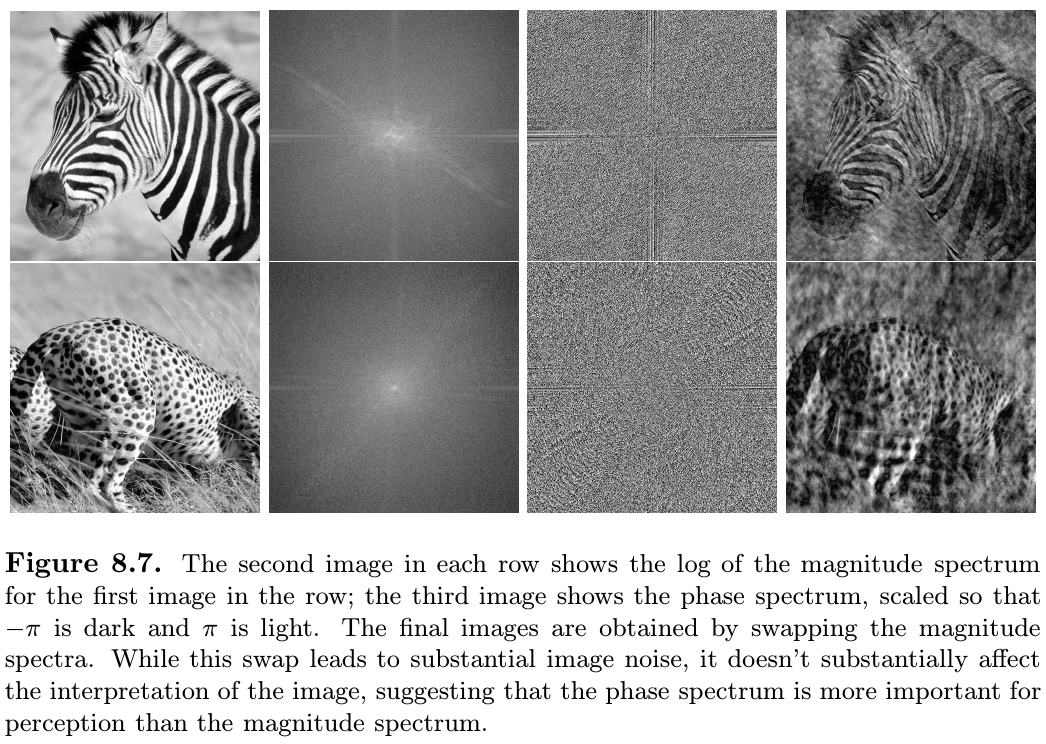
\includegraphics{img/magnitude_phase_swap.png}}
\end{frame}}{\begin{frame}
  \frametitle{采样与失真}
  
  \tmfoldedstd{{\hspace{4em}}\resizebox{0.6\columnwidth}{!}{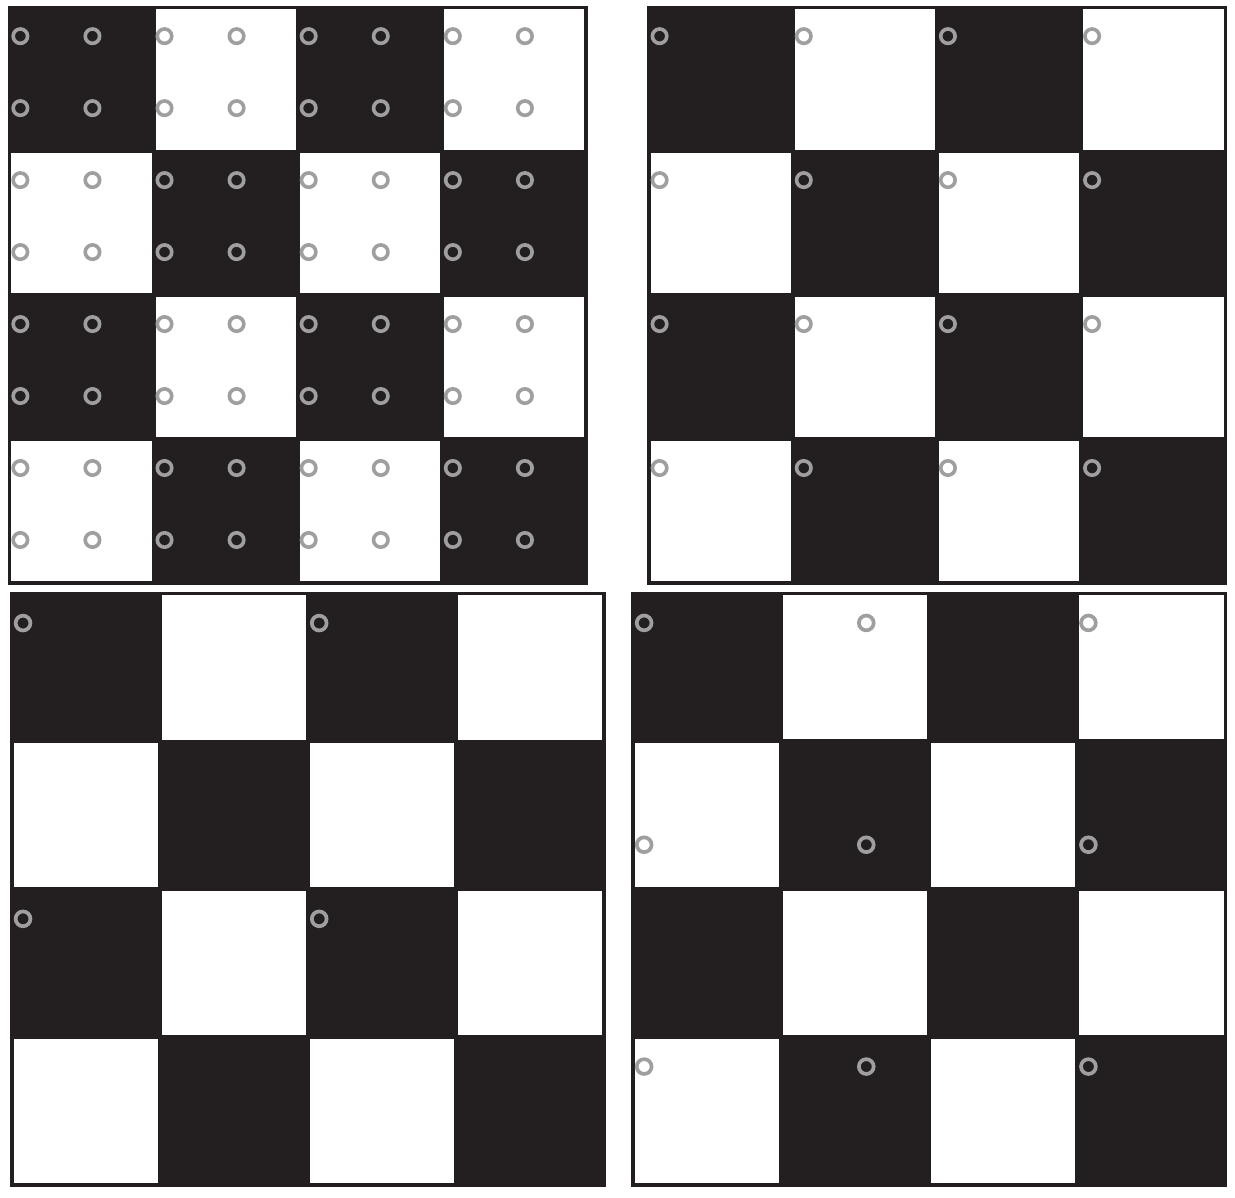
\includegraphics{img/checkboard_sampling.png}}}{Figure
  8.8. The two checkerboards on the top illustrate a sampling procedure which
  appears to be successful (whether it is or not depends on some details that
  we will deal with later). The grey circles represent the samples; if there
  are sufficient samples, then the samples represent the detail in the
  underlying function. The sampling procedure shown on the bottom is
  unequivocally unsuccessful; the samples suggest that there are fewer checks
  than there are. This illustrates two important phenomena: firstly,
  successful sampling schemes sample data ``often enough''; and, secondly,
  unsuccessful sampling schemes cause high frequency information to appear as
  lower frequency information.}
\end{frame}}{\begin{frame}
  \frametitle{一维采样}
  
  \resizebox{1\columnwidth}{!}{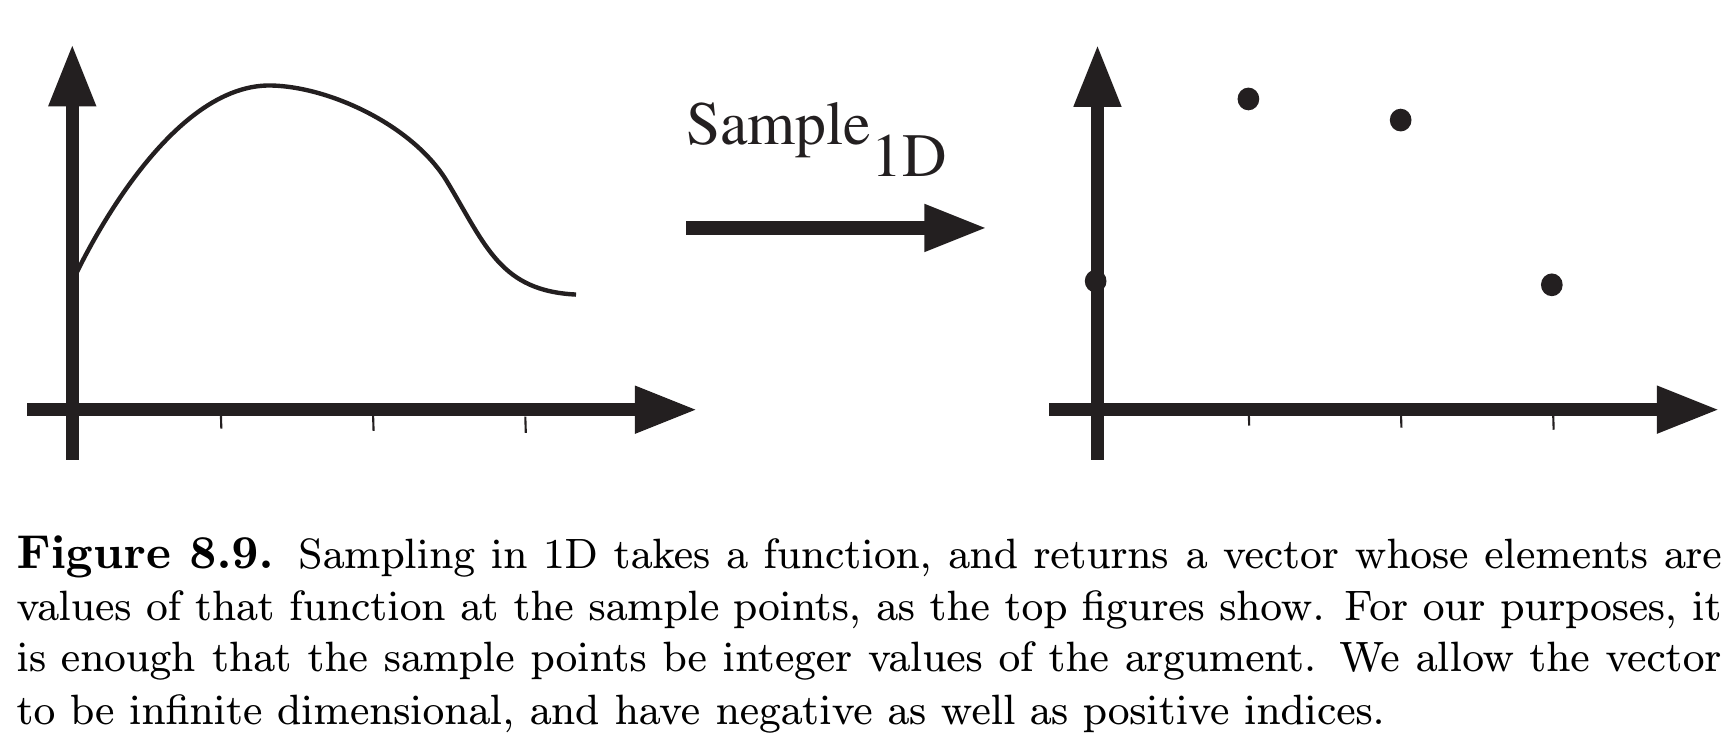
\includegraphics{img/sample1D.png}}
\end{frame}}{\begin{frame}
  \frametitle{二维采样}
  
  {\hspace{5em}}\resizebox{0.6\columnwidth}{!}{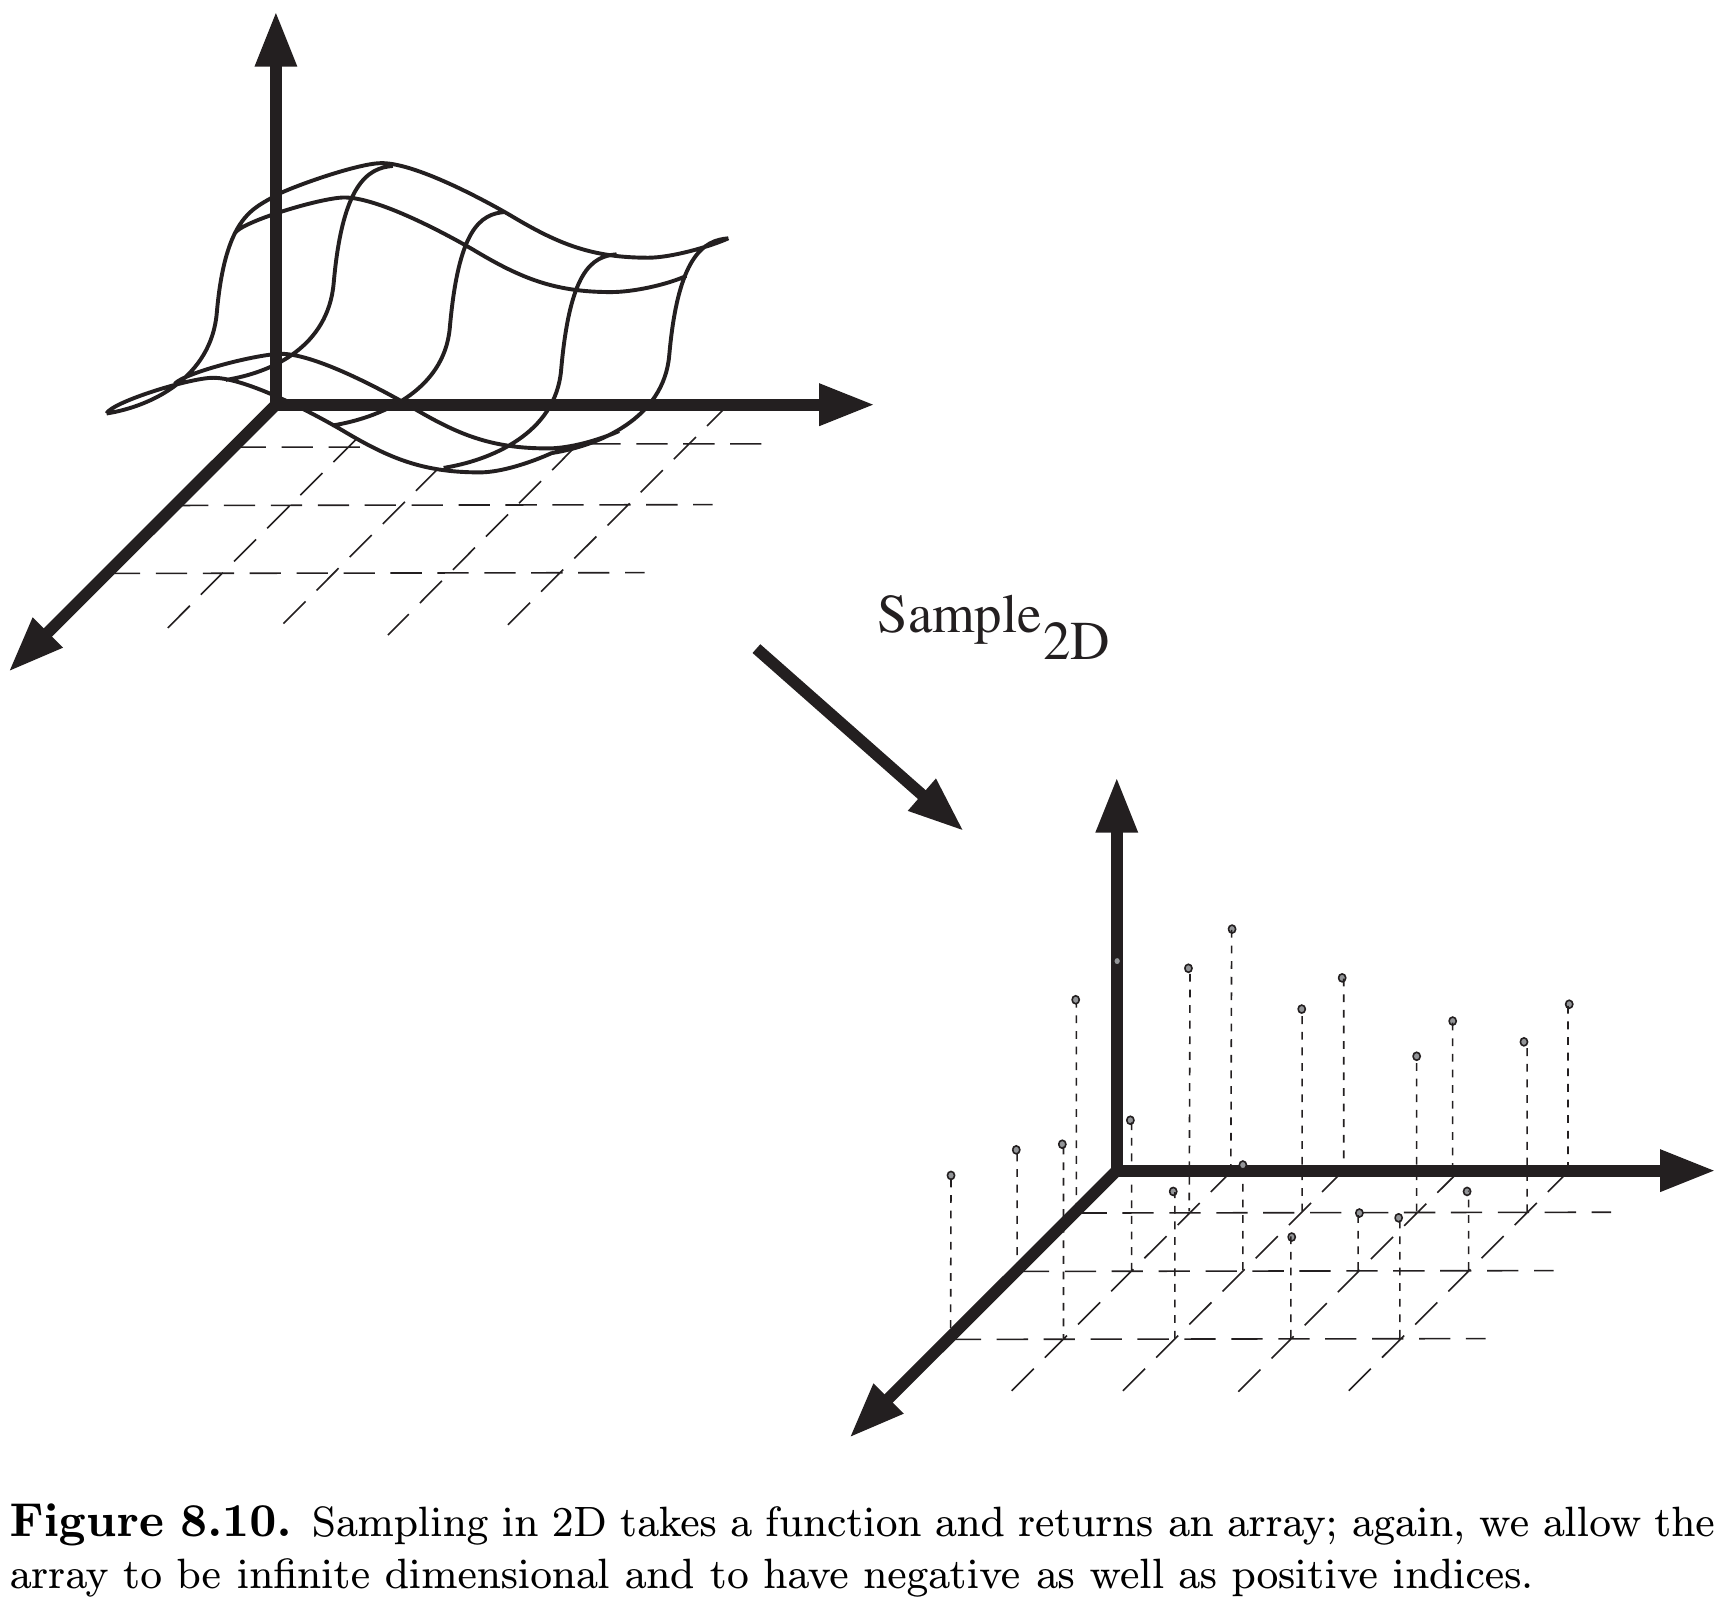
\includegraphics{img/sample2D.png}}
\end{frame}}{\begin{frame}
  \frametitle{采样信号模型}
  \begin{eqnarray*}
    \int_{- \infty}^{\infty} a \delta (x) f (x) \mathd x & = & a \nospace
    \lim_{\varepsilon \rightarrow 0} \int_{- \infty}^{+ \infty}
    d_{\varepsilon} (x) f (x) \mathd x\\
    & = & a \nospace \lim_{\varepsilon \rightarrow 0} \int_{- \infty}^{+
    \infty} \frac{\tmop{bar}_{\varepsilon} (x)}{\varepsilon} f (x) \mathd x\\
    & = & a \nospace \lim_{\varepsilon \rightarrow 0} \sum_{i = - \infty}^{+
    \infty} \frac{\tmop{bar}_{\varepsilon} (x)}{\varepsilon} f (i \varepsilon)
    \tmop{bar}_{\varepsilon} (x - i \varepsilon) \varepsilon\\
    & = & a \nospace f (0)\\
    \tmop{sample}_{2 D} (f) & = & \sum_{i = - \infty}^{\infty} \sum_{j = -
    \infty}^{\infty} f (i, j) \delta (x - i, y - j)\\
    & = & \sum_{i = - \infty}^{\infty} \sum_{j = - \infty}^{\infty} f (x, y)
    \delta (x - i, y - j)
  \end{eqnarray*}
\end{frame}}{\begin{frame}
  \
  
  
  \begin{eqnarray*}
    \mathcal{F} (\tmop{sample}_{2 D} (f (x, y))) & = & \mathcal{F} \left( f
    (x, y) \sum_{i = - \infty}^{\infty} \sum_{j = - \infty}^{\infty} \delta (x
    - i, y - j) \right)\\
    & = & \mathcal{F} (f (x, y)) \ast \ast \mathcal{F} \left( \sum_{i = -
    \infty}^{\infty} \sum_{j = - \infty}^{\infty} \delta (x - i, y - j)
    \right)\\
    & = & F (u, v) \ast \ast \sum_{i = - \infty}^{\infty} \sum_{j = -
    \infty}^{\infty} \delta (x - i, y - j)\\
    & = & \sum_{i = - \infty}^{\infty} \sum_{j = - \infty}^{\infty} F (u - i,
    v - j)
  \end{eqnarray*}
  
\end{frame}}{\begin{frame}
  \frametitle{采样信号傅里叶变换}
  
  {\hspace{5em}}\resizebox{0.7\columnwidth}{!}{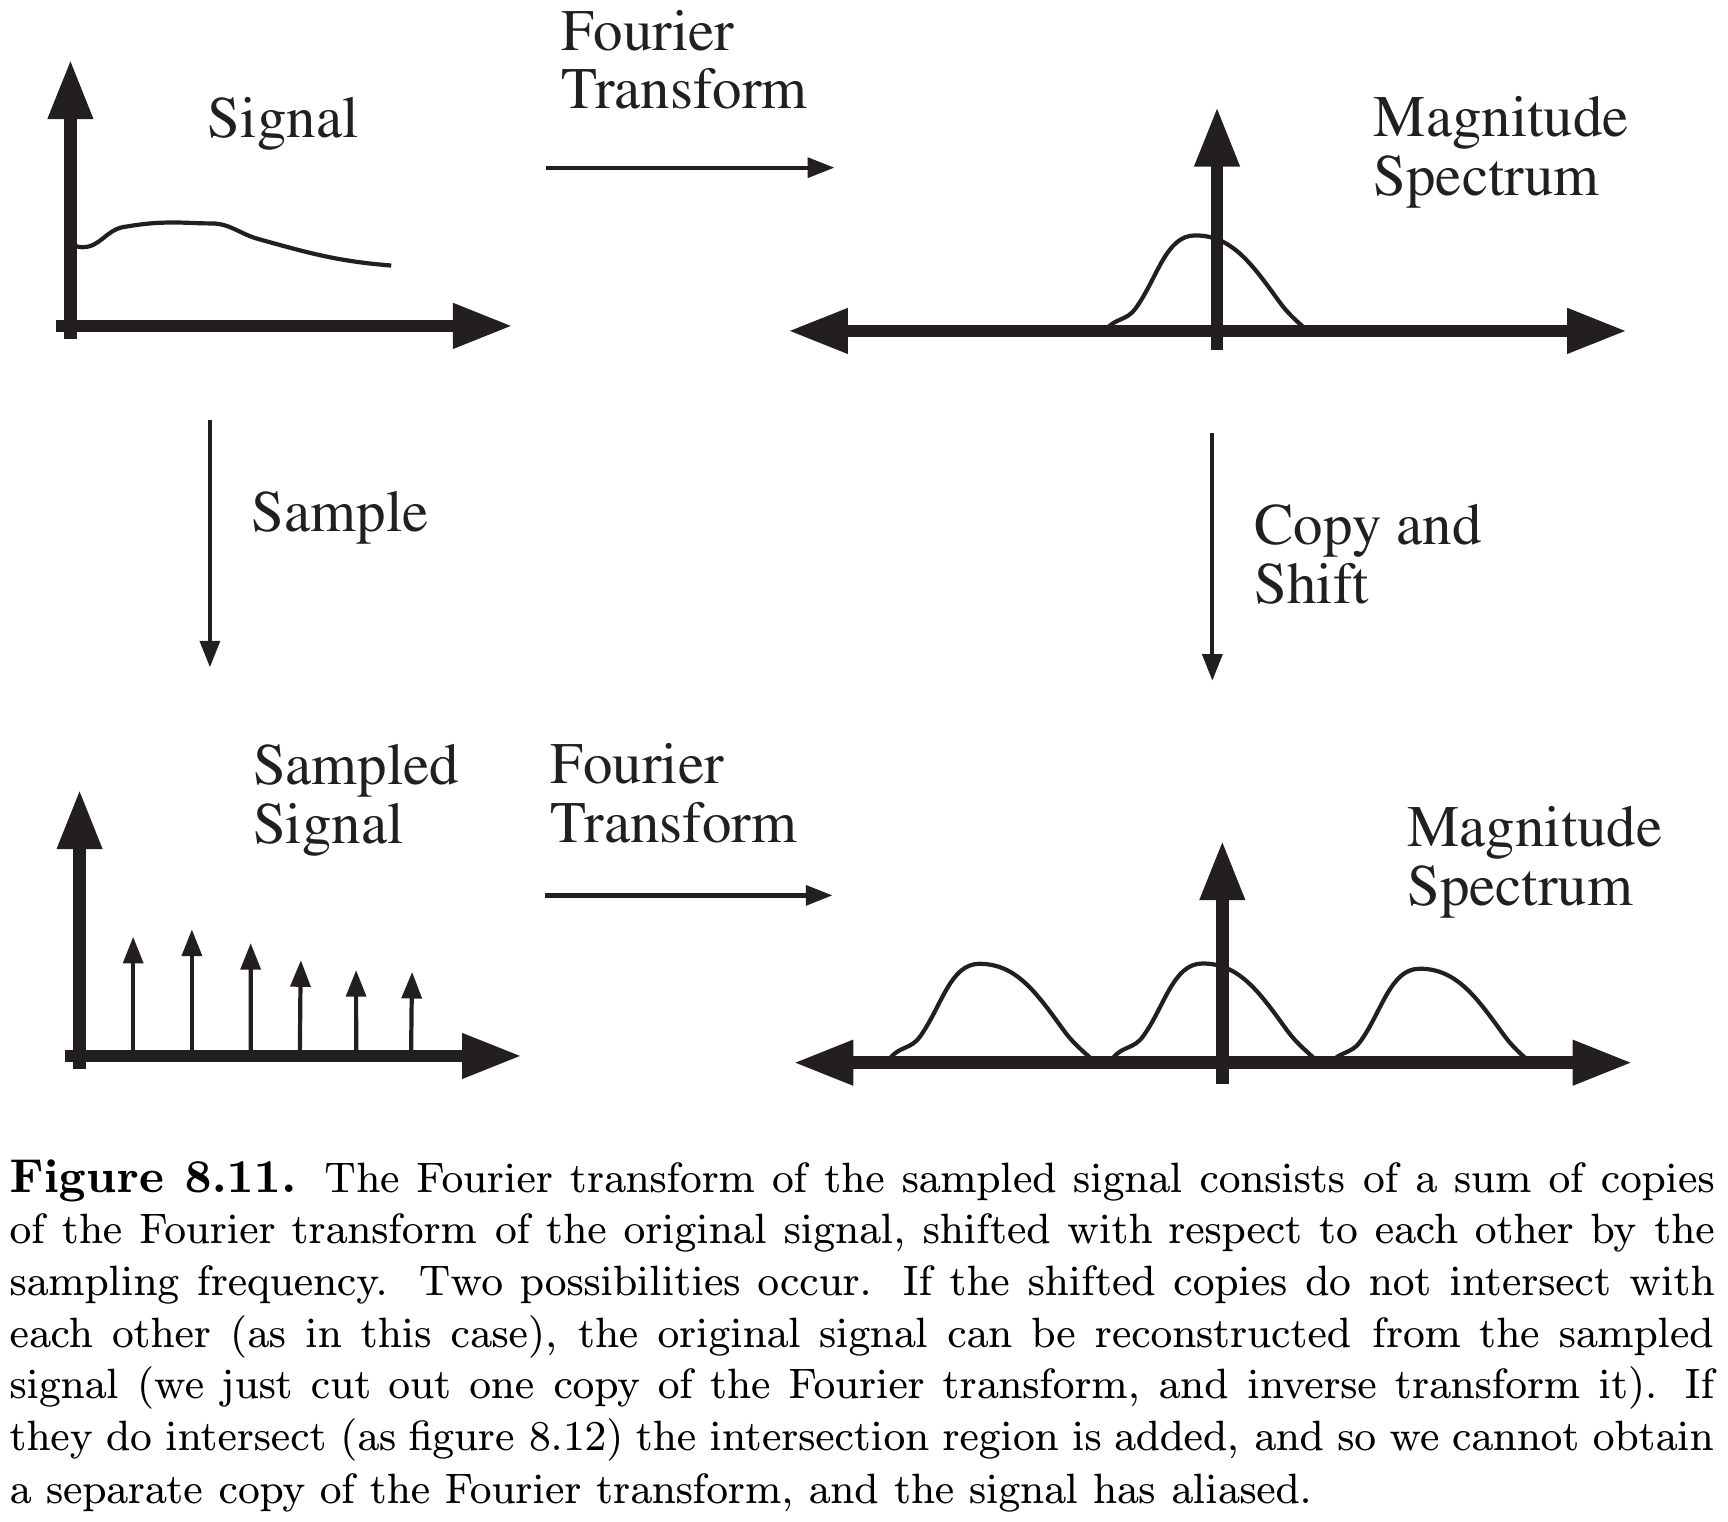
\includegraphics{img/sample_fourier1.png}}
\end{frame}}{\begin{frame}
  \frametitle{频域混叠}
  
  {\hspace{6em}}\resizebox{0.6\columnwidth}{!}{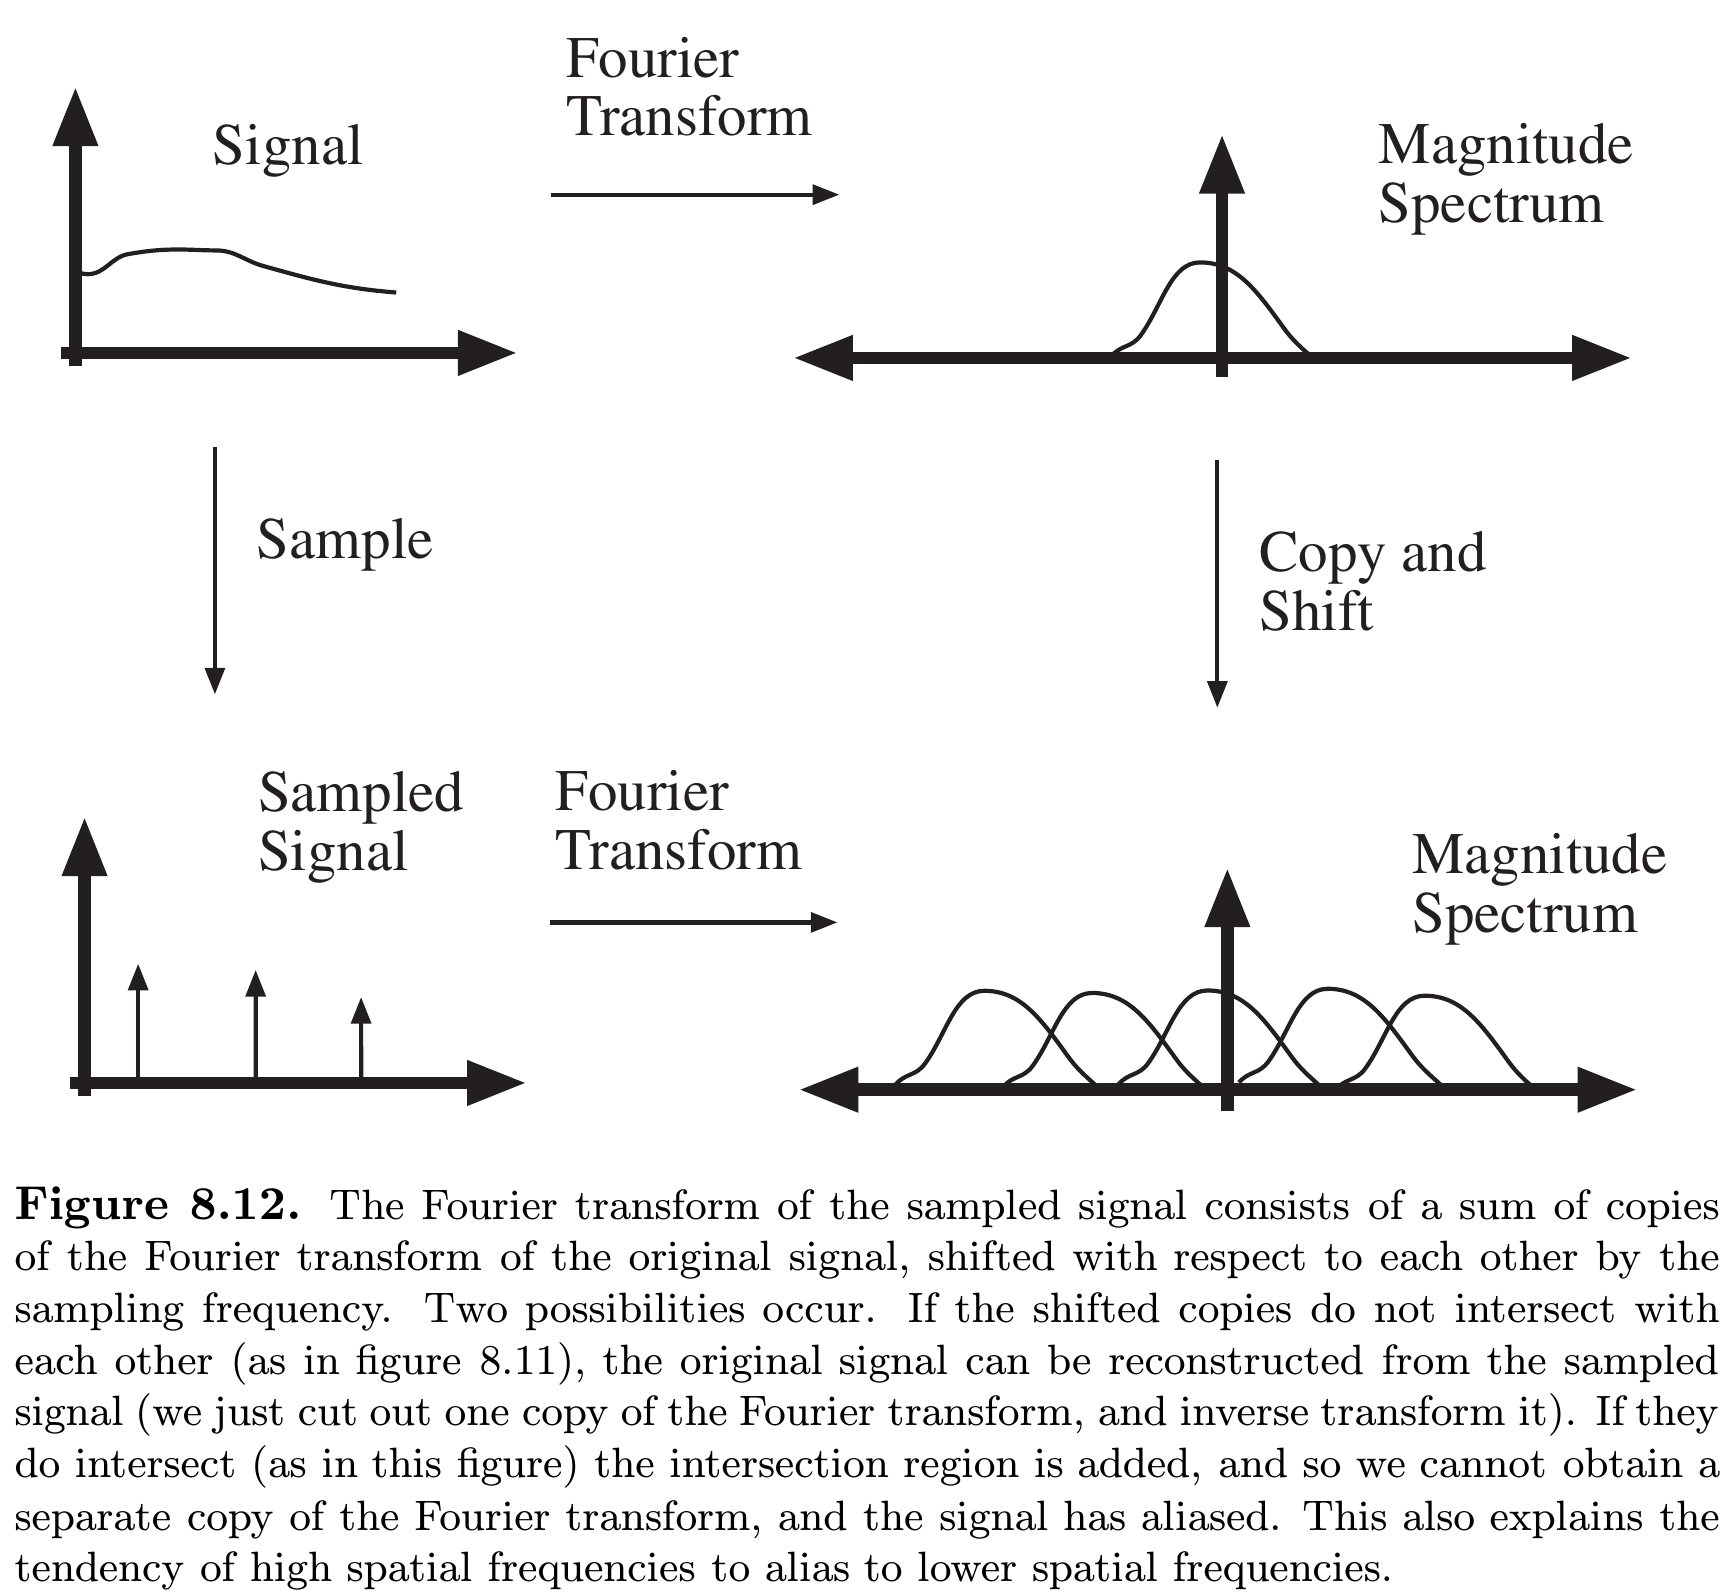
\includegraphics{img/sample_fourier_mix.png}}
\end{frame}}{\begin{frame}
  \frametitle{平采与重采样}
  
  \tmfoldedstd{\resizebox{1\columnwidth}{!}{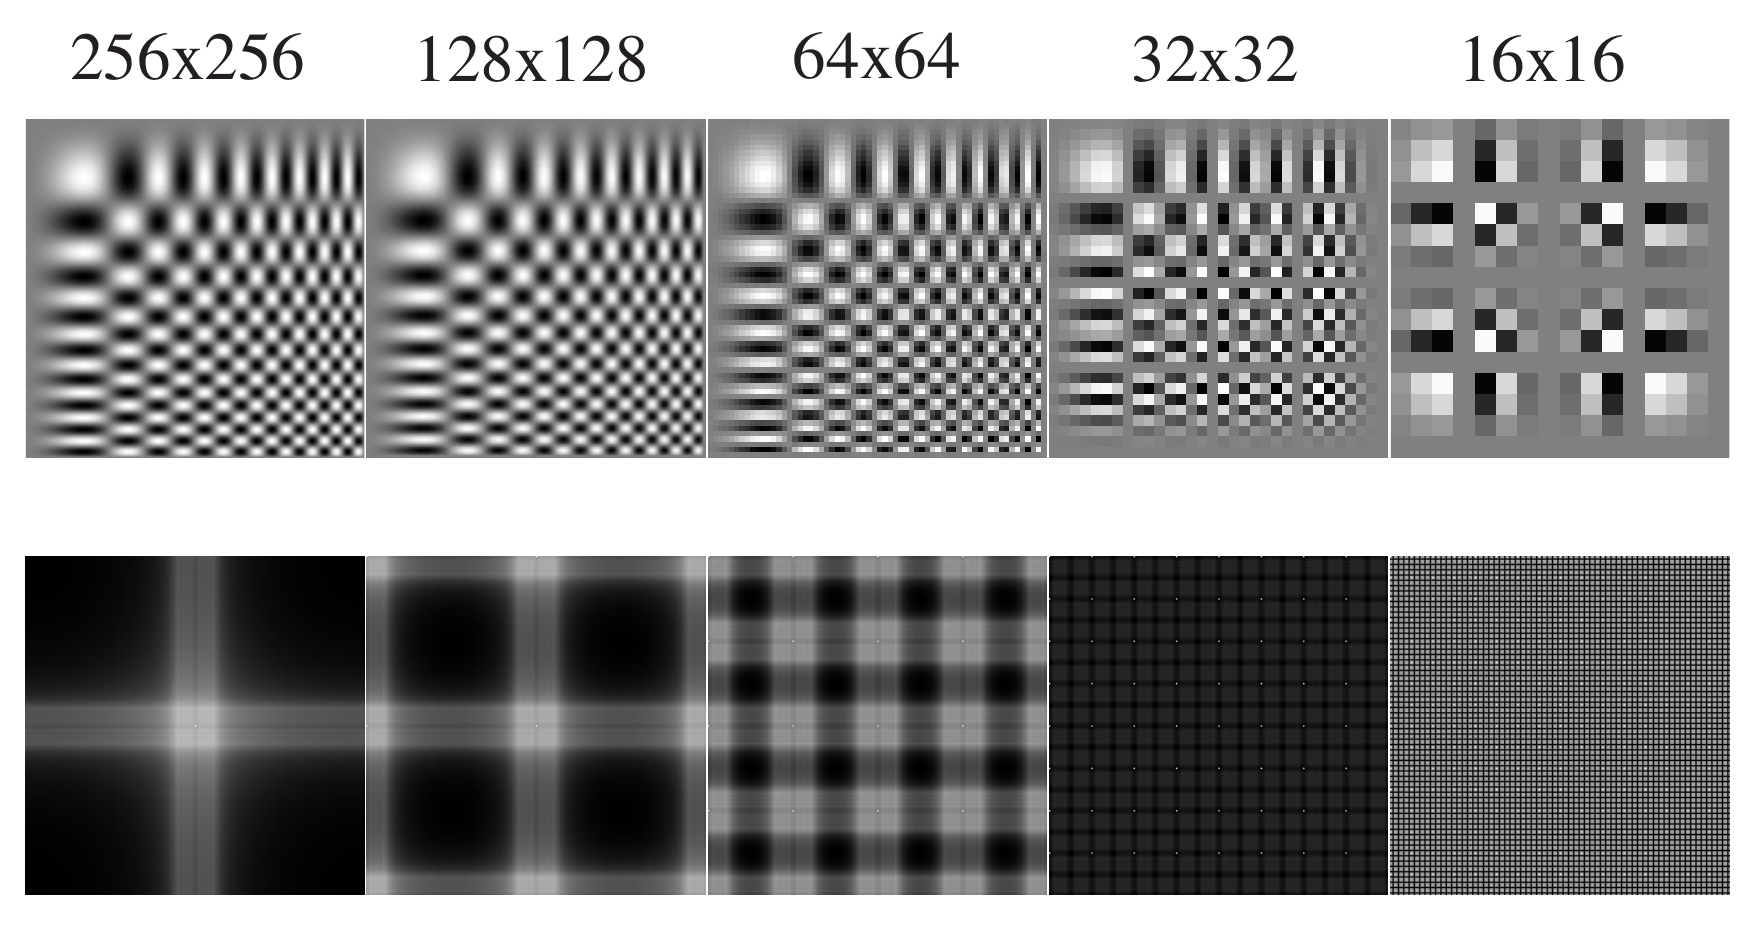
\includegraphics{img/smooth_resample_0.png}}}{Figure
  8.13. The top row shows sampled versions of an image of a grid obtained by
  multiplying two sinusoids with linearly increasing frequency --- one in x
  and one in y. The other images in the series are obtained by resampling by
  factors of two, without smoothing (i.e. the next is a 128x128, then a 64x64,
  etc., all scaled to the same size). Note the substantial aliasing; high
  spatial frequencies alias down to low spatial frequencies, and the smallest
  image is an extremely poor representation of the large image. The bottom row
  shows the magnitude of the Fourier transform of each image --- displayed as
  a log, to compress the intensity scale. The constant component is at the
  center. Notice that the Fourier transform of a resampled image is obtained
  by scaling the Fourier transform of the original image and then tiling the
  plane. Interference between copies of the original Fourier transform means
  that we cannot recover its value at some points --- this is the mechanism
  underlying aliasing.
  
  \ }
\end{frame}}{\begin{frame}
  \frametitle{平滑与重采样(高斯平滑)}
  
  {\hspace{3em}}\resizebox{0.8\columnwidth}{!}{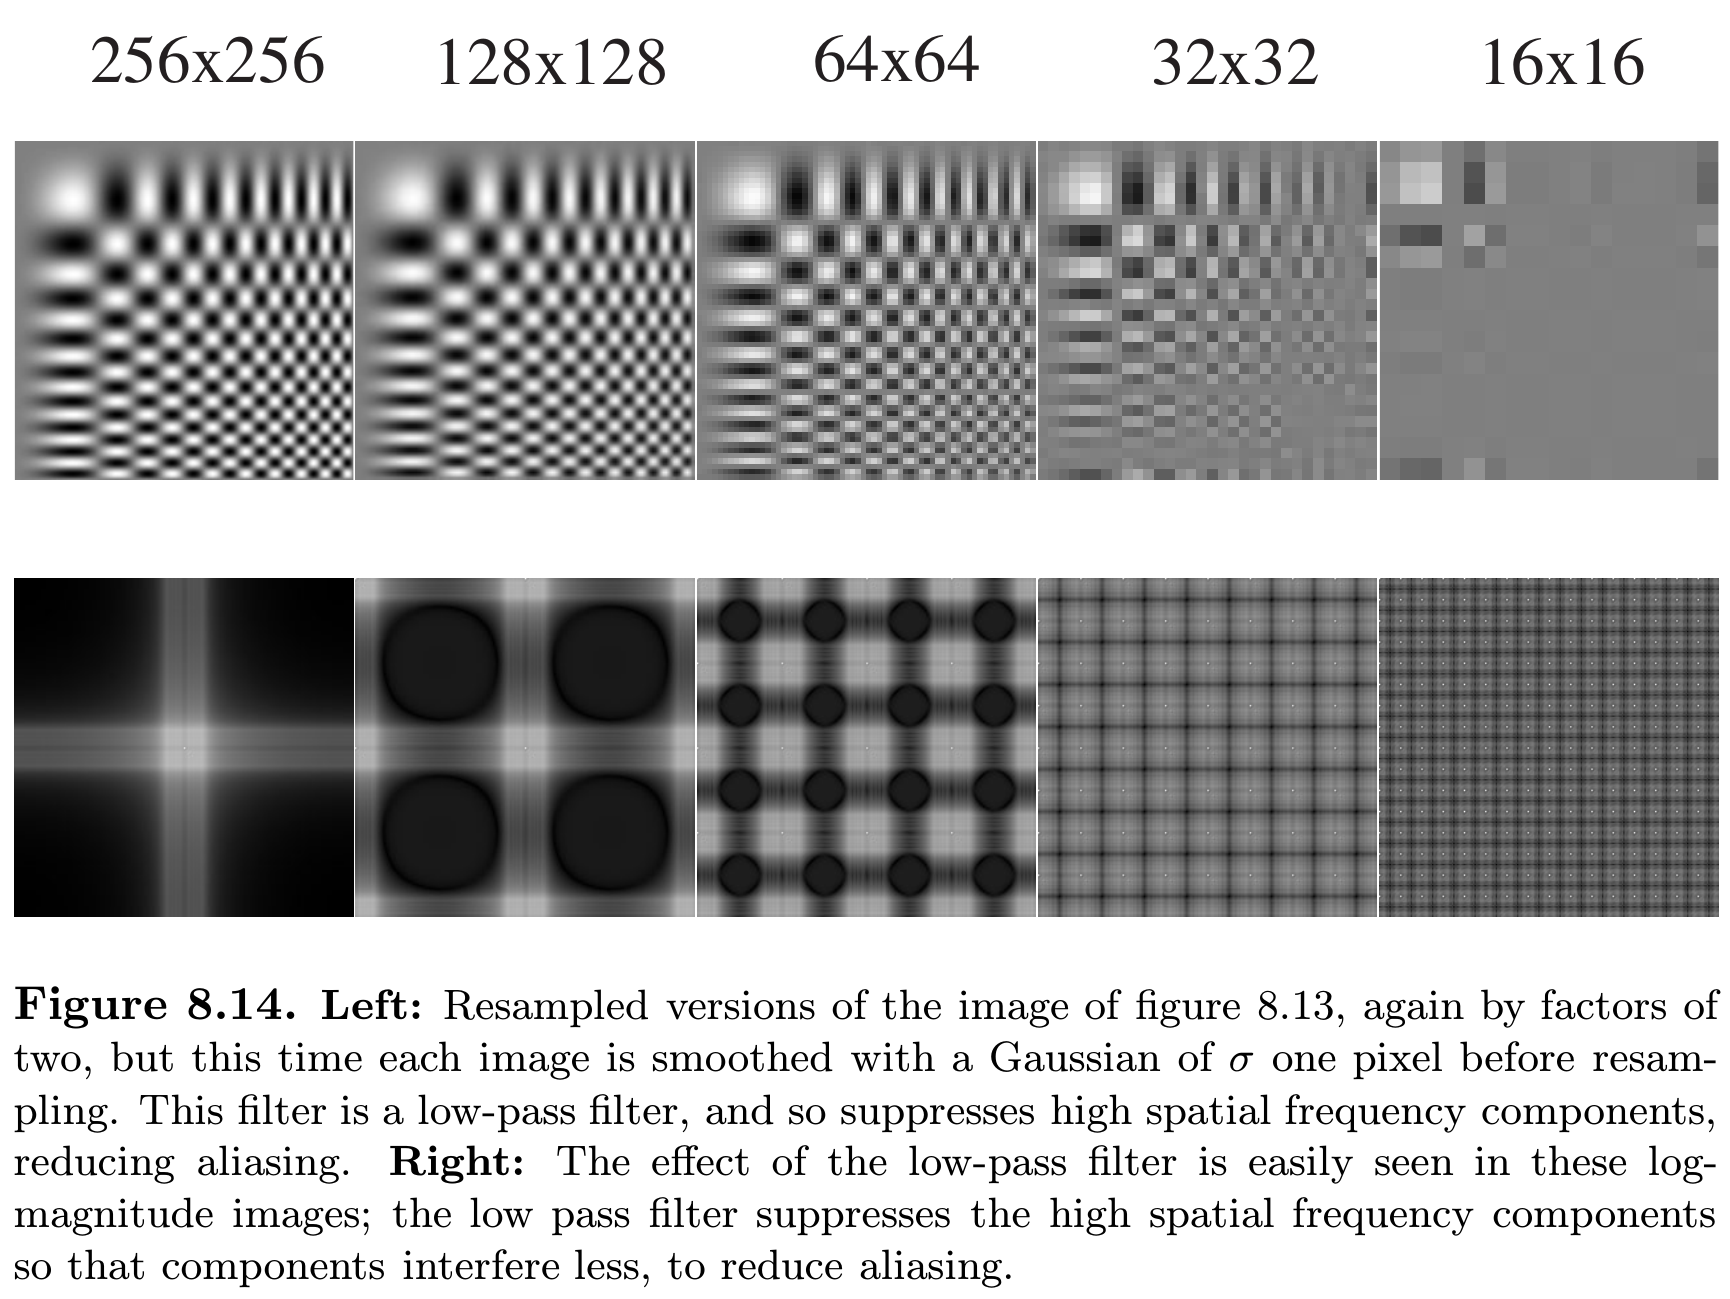
\includegraphics{img/smooth_resample_1.png}}
\end{frame}}{\begin{frame}
  \frametitle{平滑与重采样(高斯平滑)}
  
  \qquad\resizebox{0.8\columnwidth}{!}{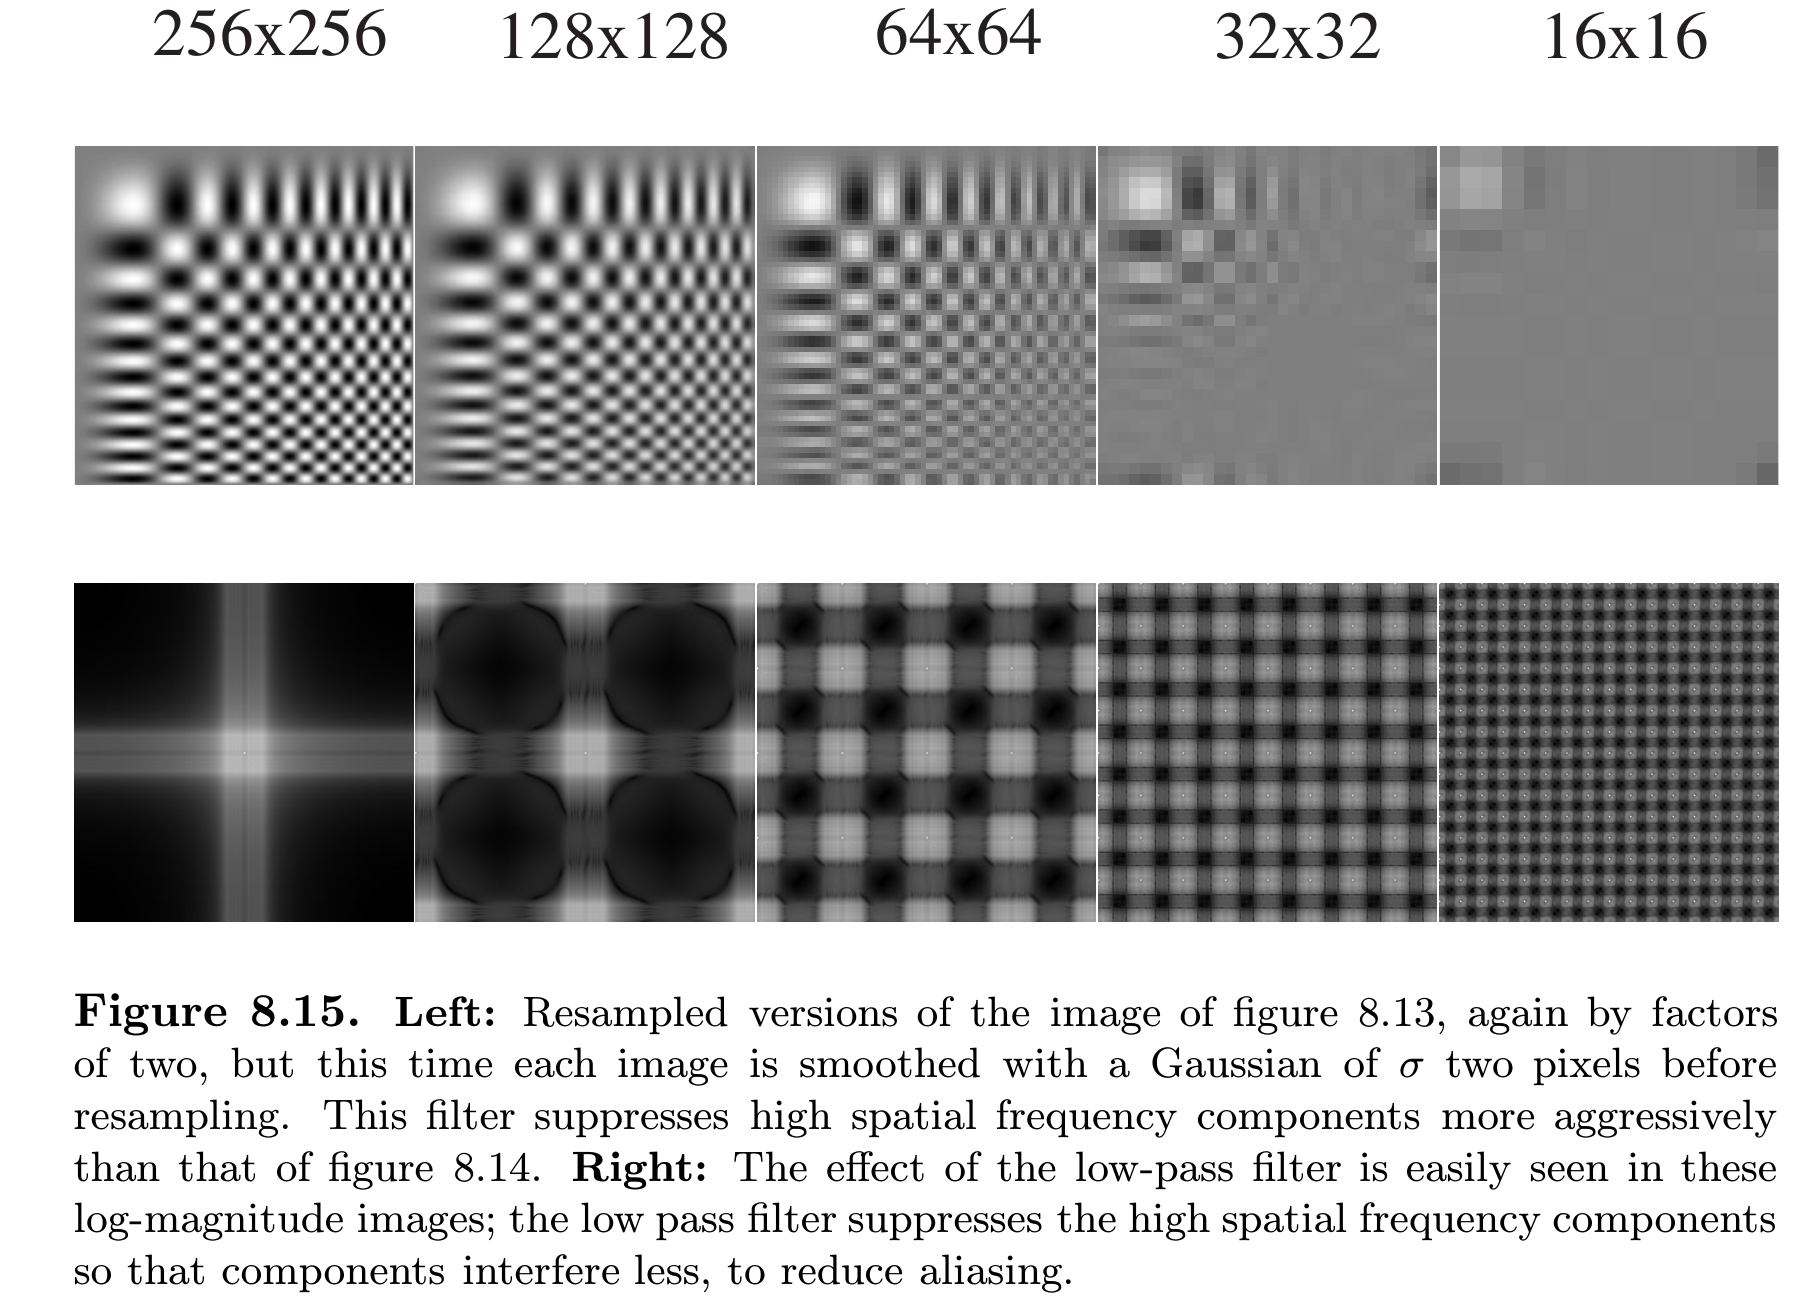
\includegraphics{img/smooth_resample_2.png}}
\end{frame}}{\frametitle{高斯金字塔}

{\hspace{7em}}\resizebox{0.5\columnwidth}{!}{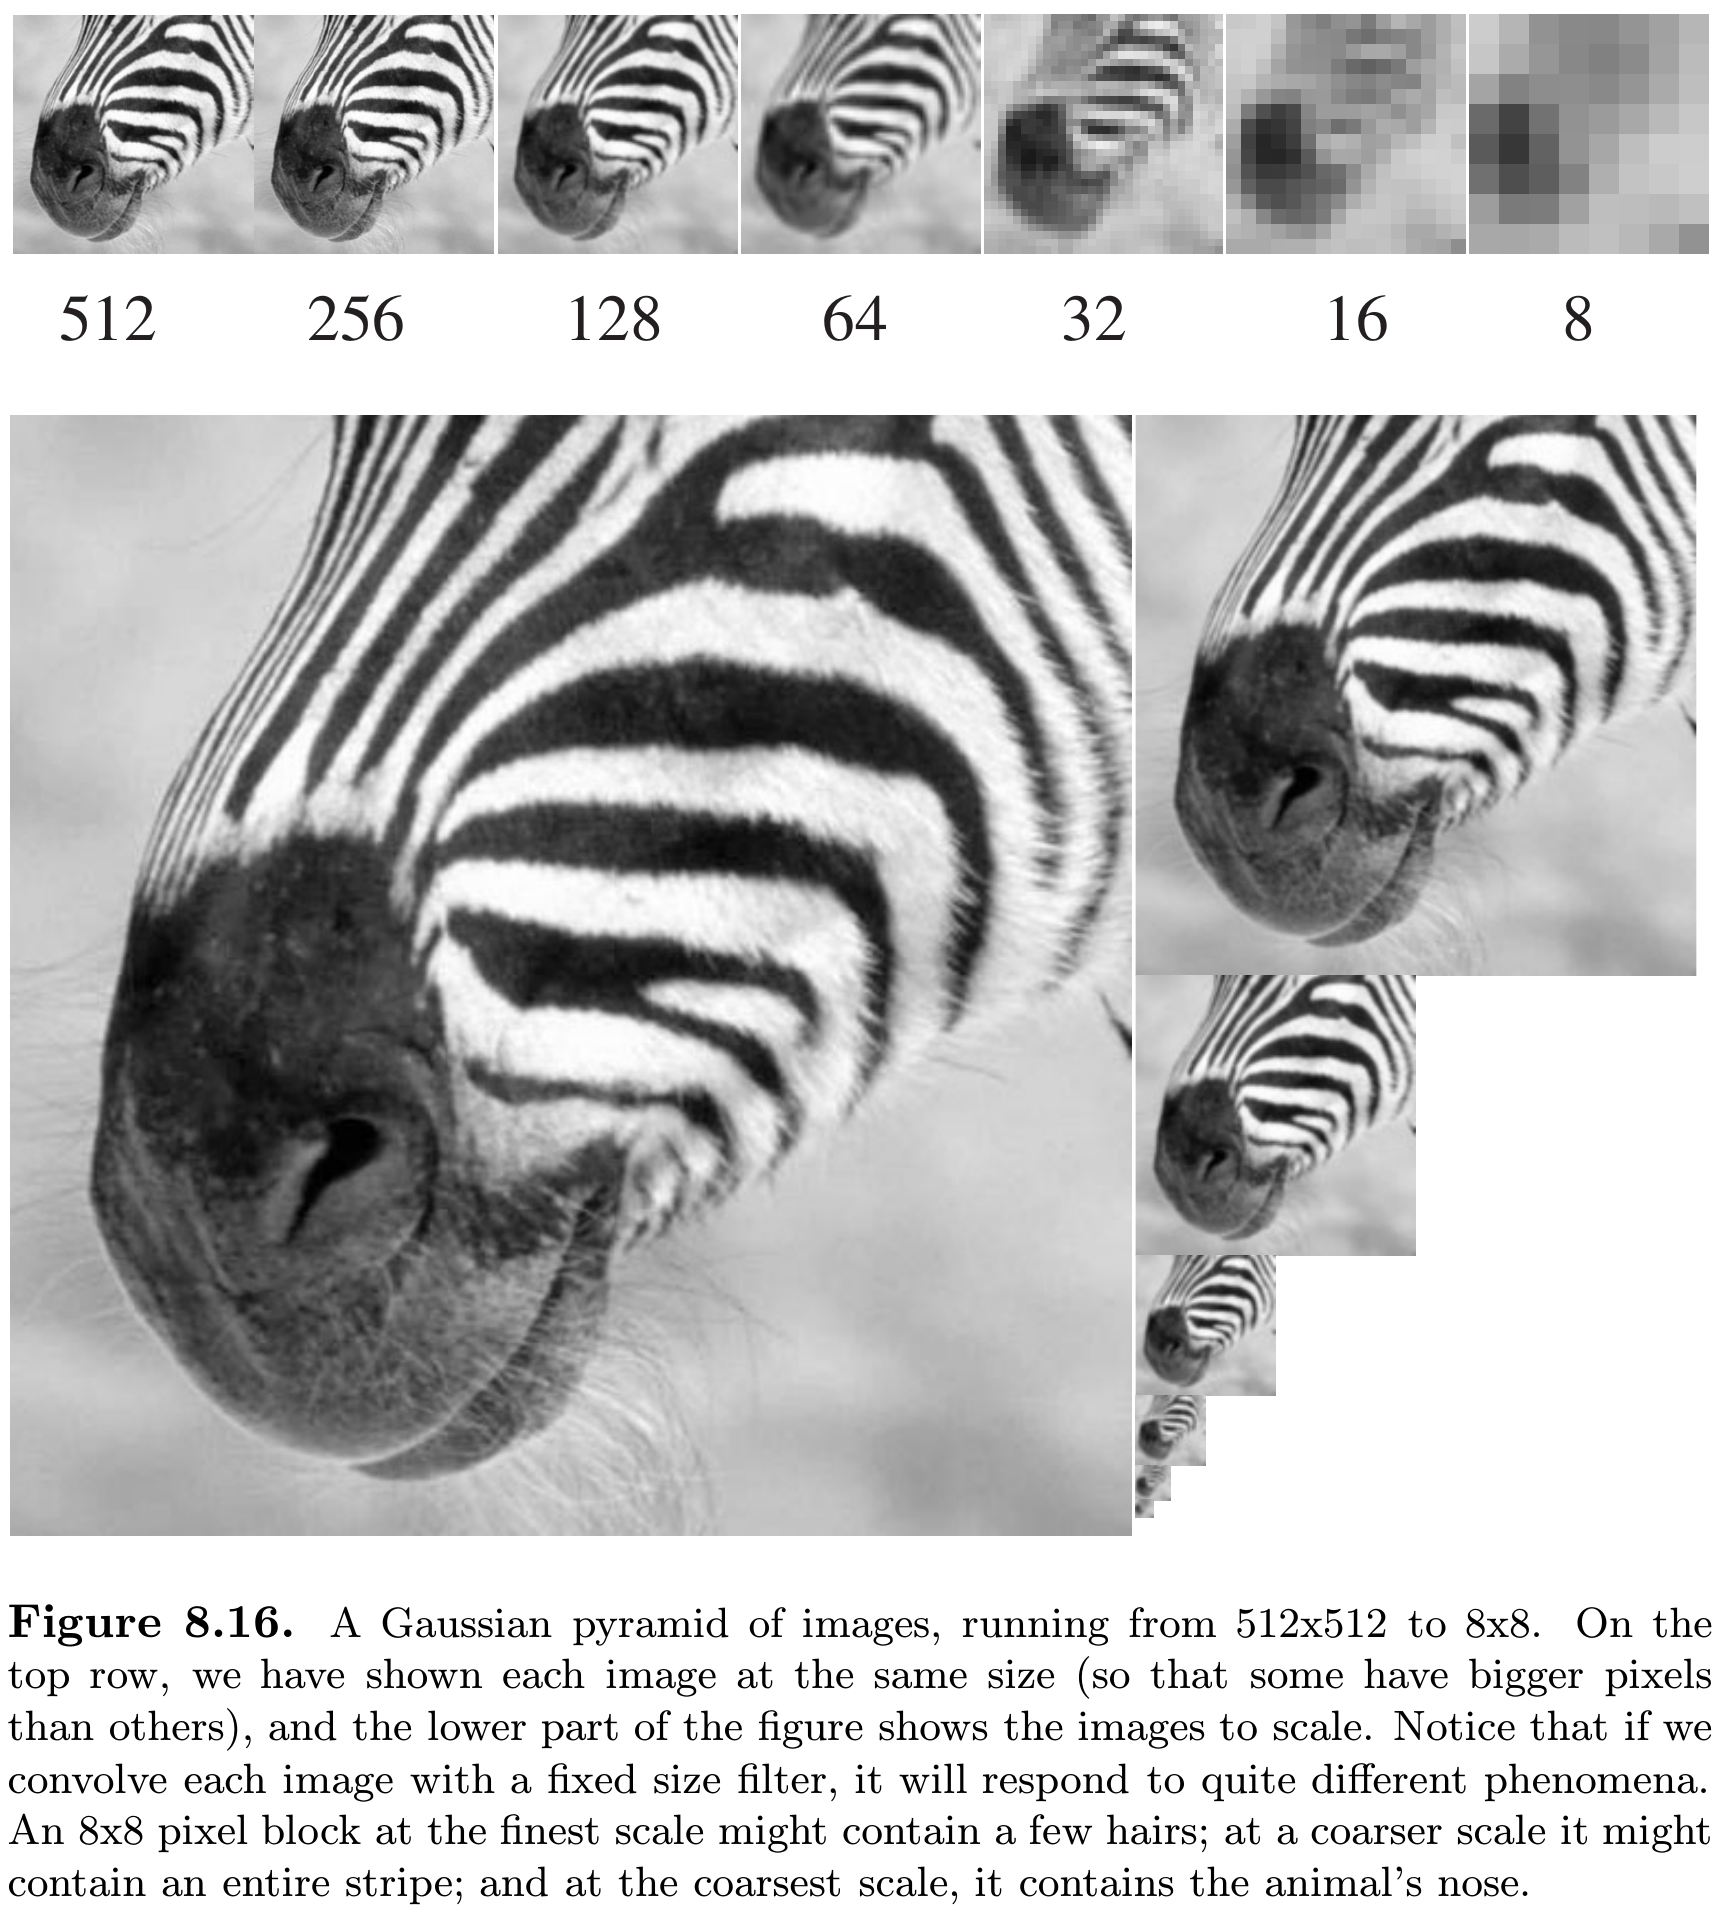
\includegraphics{img/gaussian_pyramid.png}}}{\begin{frame}
  \frametitle{尺度空间}
  
  {\hspace{5em}}\resizebox{0.6\columnwidth}{!}{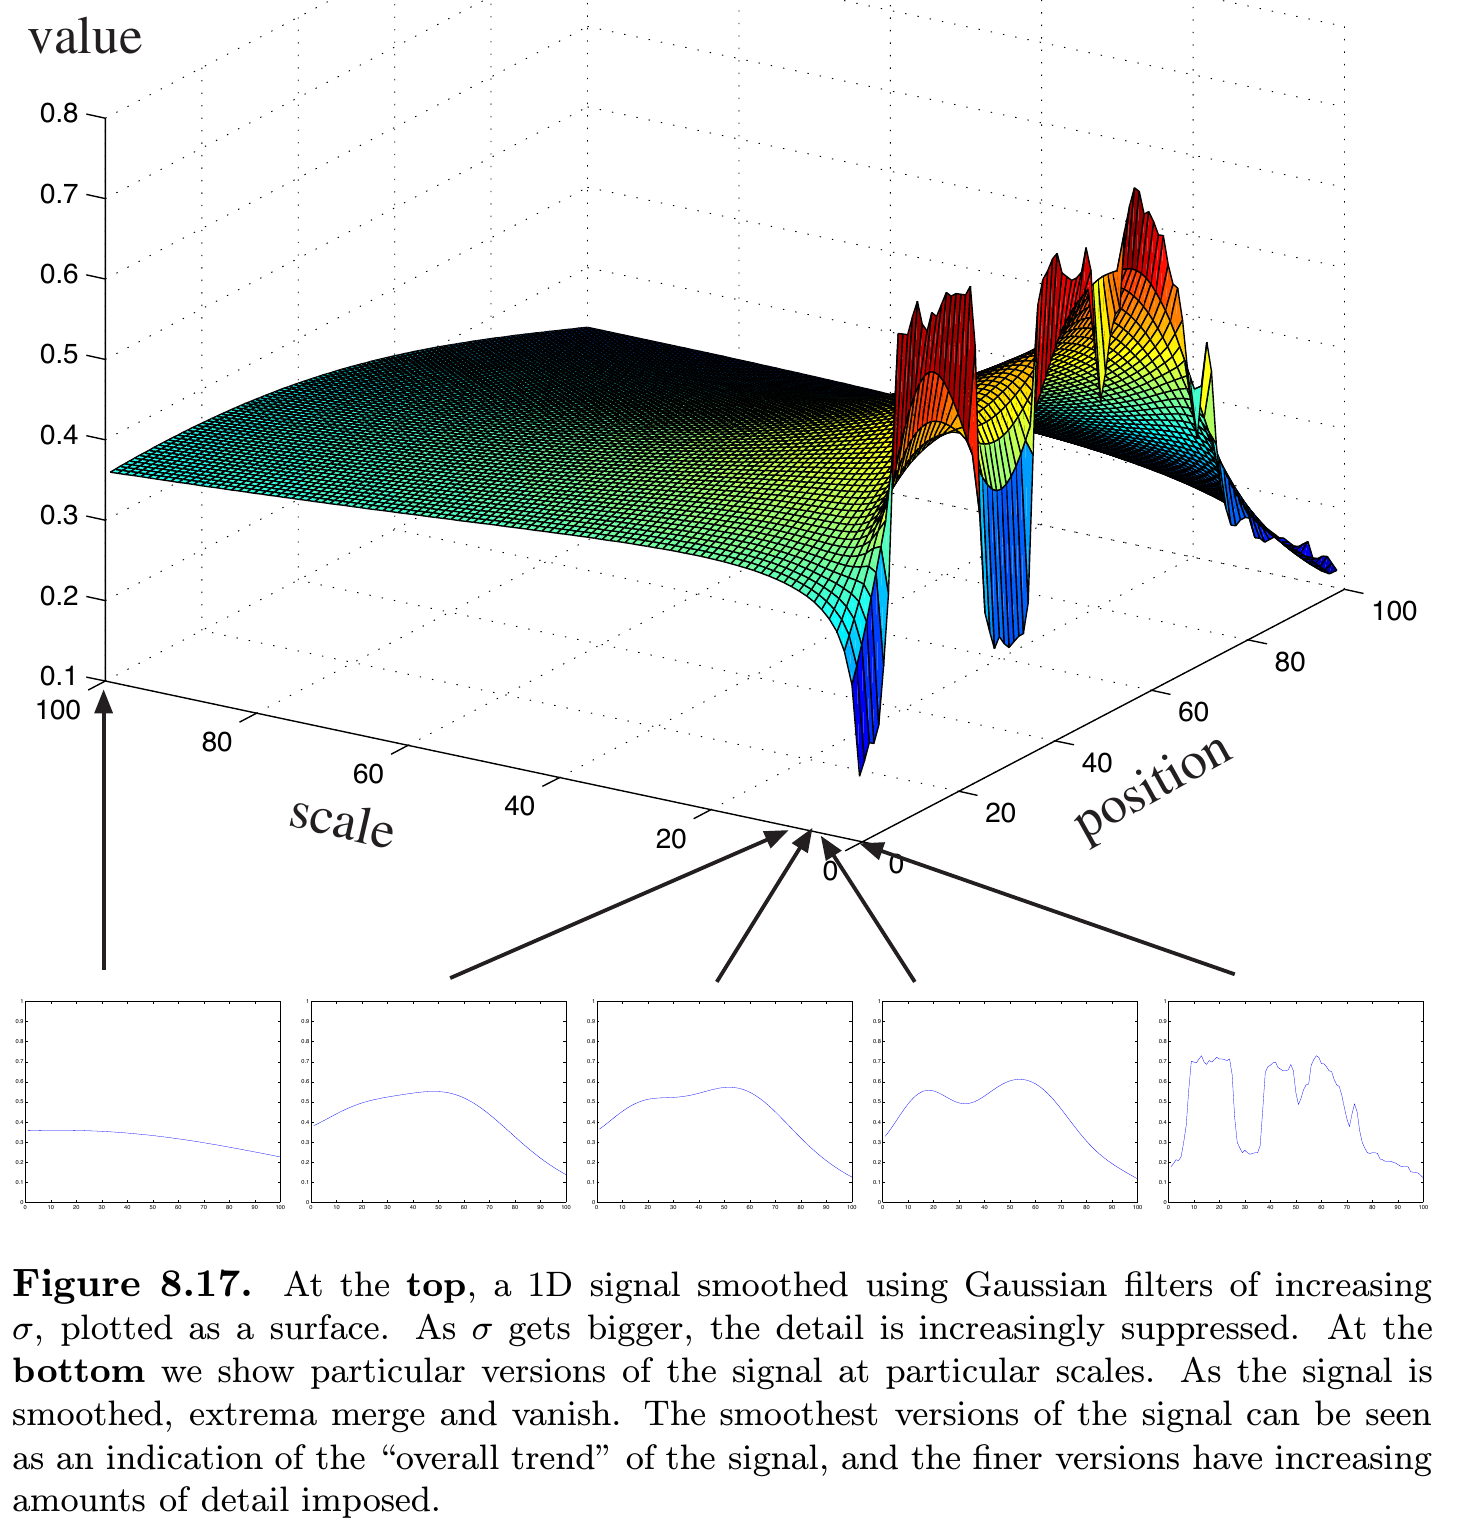
\includegraphics{img/scale_space.png}}
\end{frame}}{\begin{frame}
  \frametitle{Zero-crossing}
  
  {\hspace{5em}}\resizebox{0.6\columnwidth}{!}{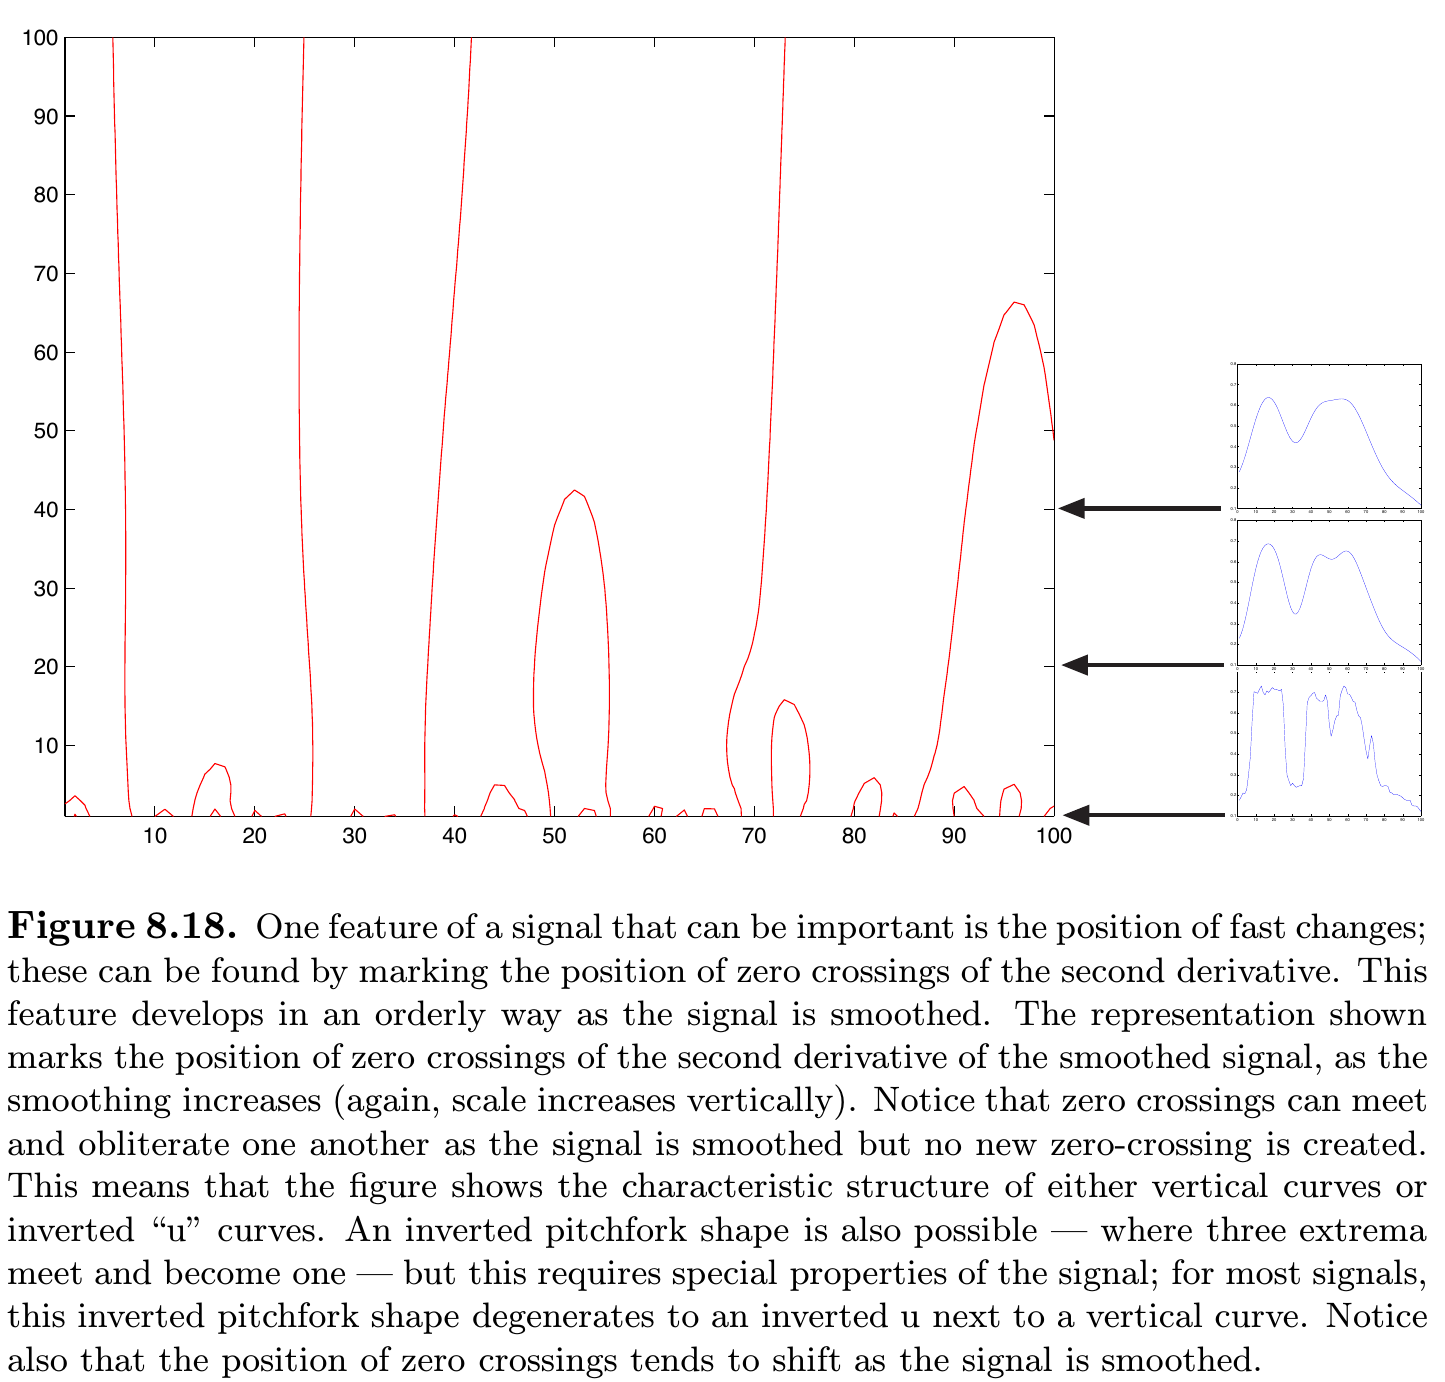
\includegraphics{img/zero_crossing.png}}
\end{frame}}{\begin{frame}
  \frametitle{2D}
  
  \resizebox{1\columnwidth}{!}{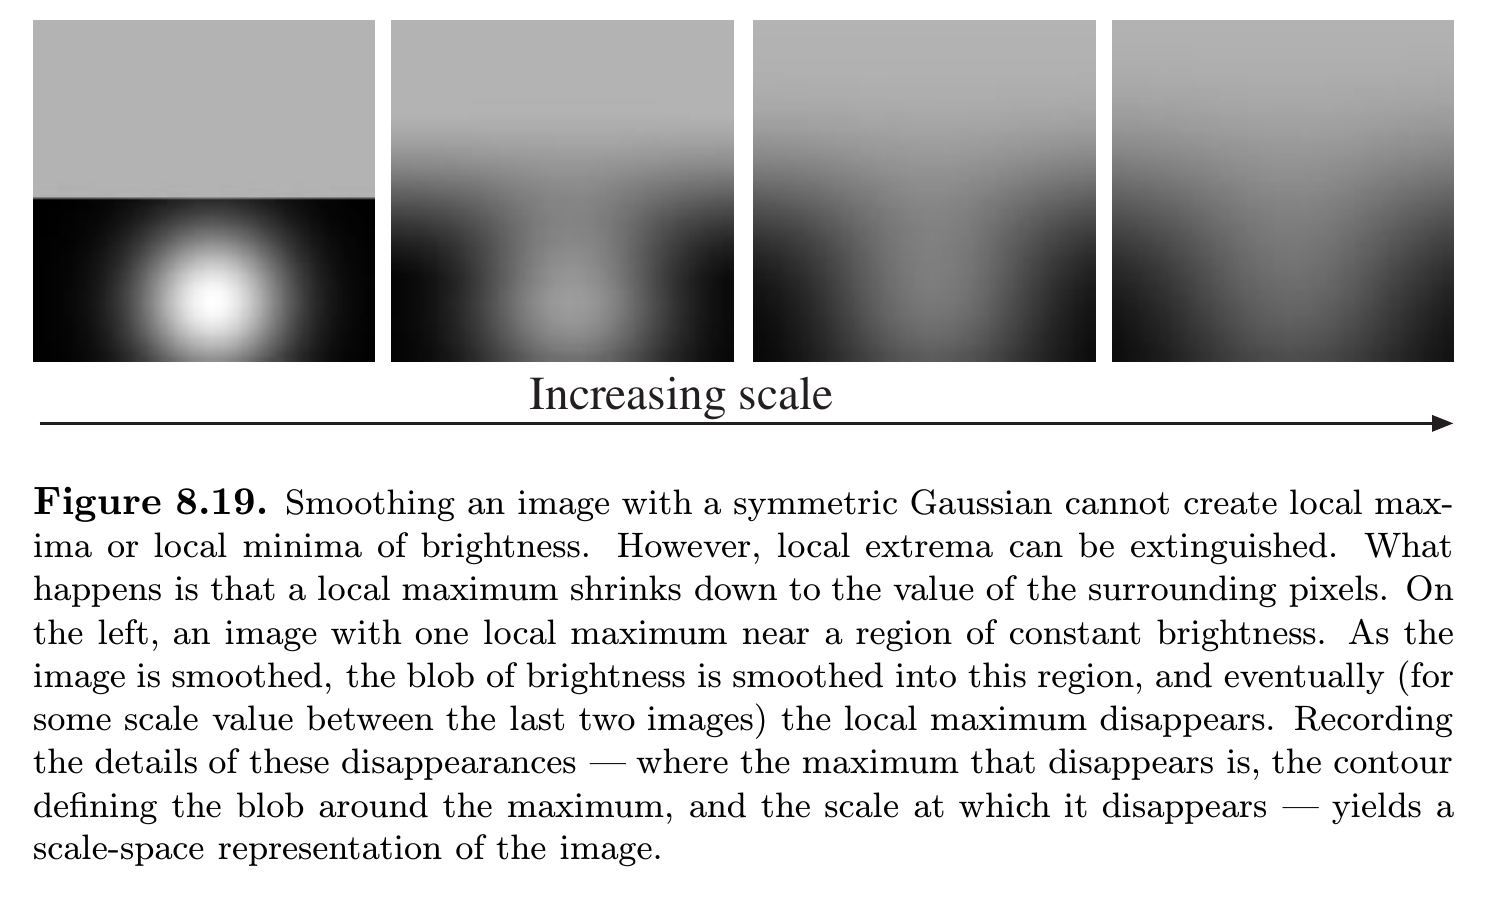
\includegraphics{img/scale_space_2D.png}}
\end{frame}}}

\end{document}
